\chapter{Day 3 Nonlinearities}
\label{ch-day3}





% ******************************************************************
% ******************************************************************
% ******************************************************************
\clearpage
\newpage
\section{Single element Models: illustrate the elastic-plastic behavior}
\label{Single_element_Models_illustrate_the_elastic-plastic_behavior}
\subsection{von-Mises material model}


\paragraph{von-Mises perfectly plastic material model}
The Real-ESSI input files for von-Mises perfectly plastic example are available 
\href{http://cml01.engr.ucdavis.edu/shortCourse/Day3/Single_element_Models_illustrate_the_elastic-plastic_behavior/vmpp}{HERE}. 
The compressed package of Real-ESSI input files for this example is available 
\href{http://cml01.engr.ucdavis.edu/shortCourse/Day3/Single_element_Models_illustrate_the_elastic-plastic_behavior/vmpp/vmpp.tgz}{HERE}. 

\paragraph{von-Mises Armstrong-Frederick material model}
The Real-ESSI input files for von-Mises Armstrong-Frederick example are available 
\href{http://cml01.engr.ucdavis.edu/shortCourse/Day3/Single_element_Models_illustrate_the_elastic-plastic_behavior/vmaf}{HERE}. 
The compressed package of Real-ESSI input files for this example is available 
\href{http://cml01.engr.ucdavis.edu/shortCourse/Day3/Single_element_Models_illustrate_the_elastic-plastic_behavior/vmaf/vmaf.tgz}{HERE}. 


The Modeling parameters are listed.
\begin{itemize}
  \item Left: von-Mises linear hardening material model 
  \begin{itemize}
    \item Mass Density, $\rho$, \enspace \enspace 0.0 $kg/m^3$
    \item Young's modulus, $E$, \enspace \enspace 20 MPa
    \item Poisson's ratio, $\nu$, \enspace \enspace 0.0
    \item von Mises radius, $k$, \enspace \enspace 100 kPa
    \item kinematic hardening rate, $K_{kine} $, \enspace \enspace 2 MPa
    \item isotropic hardening rate, $K_{iso} $, \enspace \enspace 0 Pa
  \end{itemize}
  \item Right: Drucker-Prager nonlinear hardening material model 
  \begin{itemize}
    \item Mass Density, $\rho$, \enspace \enspace 0.0 $kg/m^3$
    \item Young's modulus, $E$, \enspace \enspace 20 MPa
    \item Poisson's ratio, $\nu$, \enspace \enspace 0.0
    \item Drucker-Prager, $k$, \enspace \enspace 0.179527
    \item nonlinear kinematic hardening, $H_a$, \enspace \enspace 20 MPa
    \item nonlinear kinematic hardening, $C_r$, \enspace \enspace 100
    \item isotropic hardening rate, $K_{iso} $, \enspace \enspace 0 Pa
    \item initial confining stress, $p_0$, \enspace \enspace 1 Pa
  \end{itemize}
\end{itemize}

\begin{figure}[H]
  \centering
  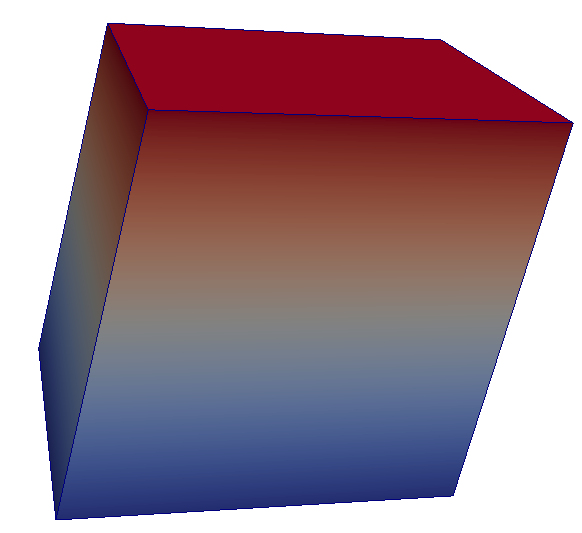
\includegraphics[width = 6cm]{./Figure-files/Day3/Single_element_Models_illustrate_the_elastic-plastic_behavior/overview.png}
  \caption{Simulation Model of Single Element}
  \label{fig_single_element_elastic_plastic1}
\end{figure}


The illustration results are shown in Fig.~\ref{fig_single_element_elastic_plastic_vmpp_vmaf}.

\begin{figure}[H]
  \centering
  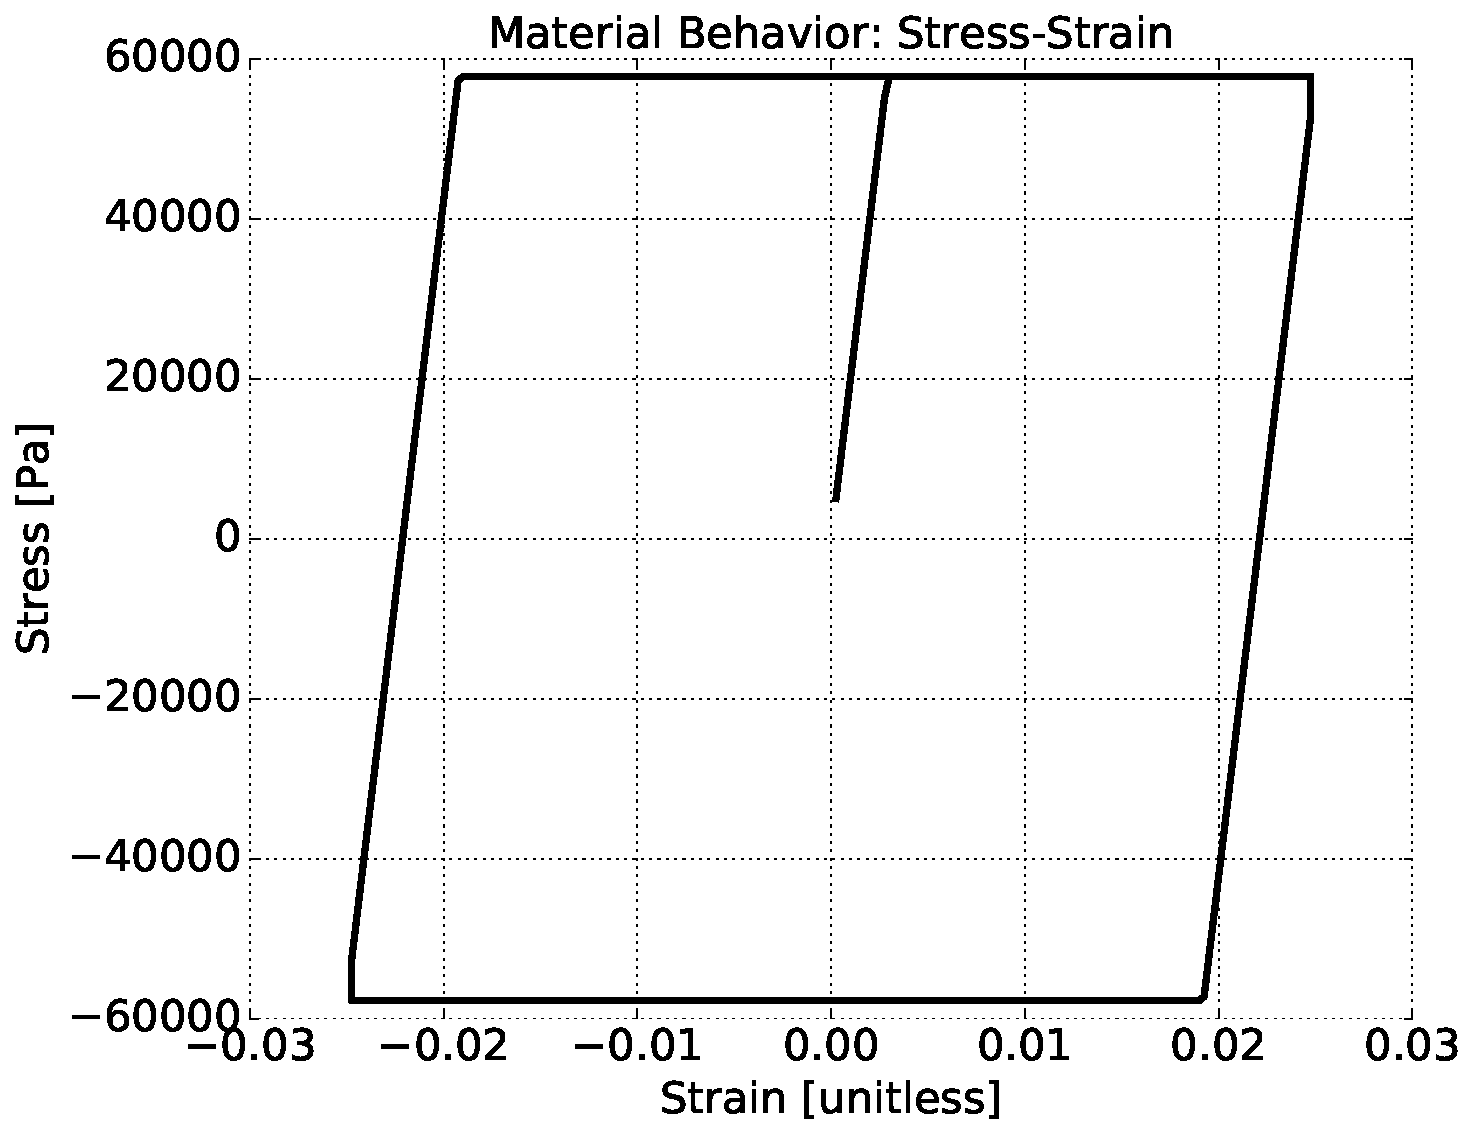
\includegraphics[width = 7cm]{./Figure-files/Day3/Single_element_Models_illustrate_the_elastic-plastic_behavior/vmpp.pdf}
  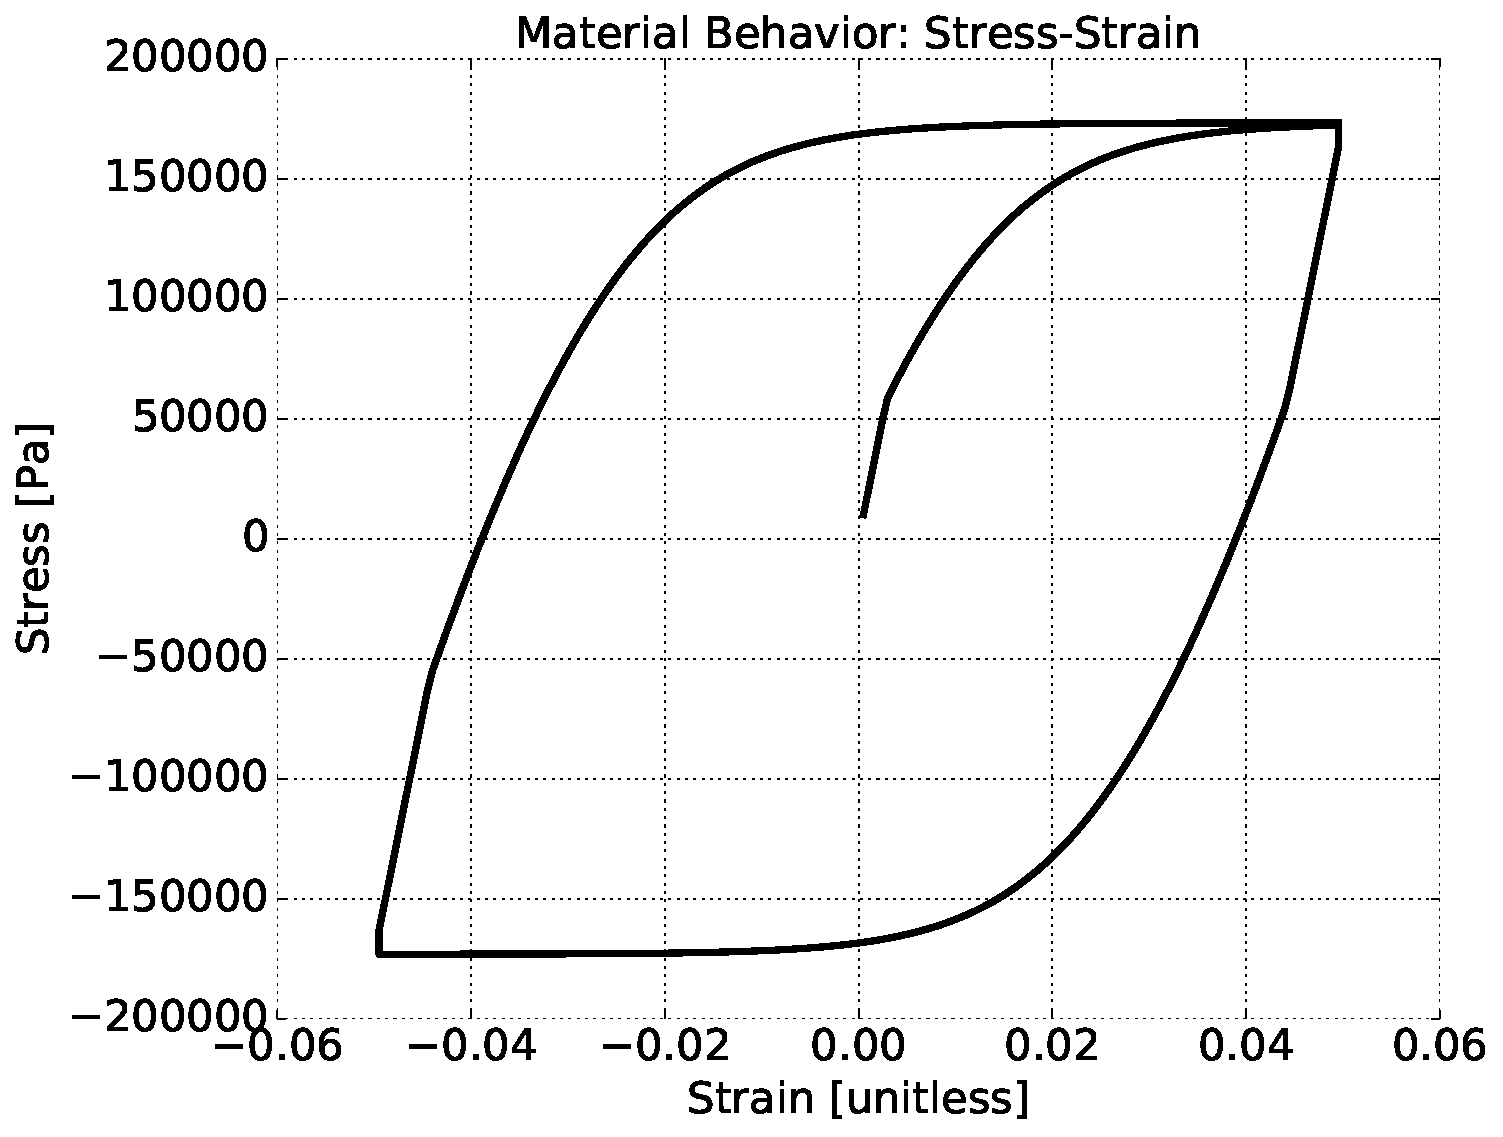
\includegraphics[width = 7cm]{./Figure-files/Day3/Single_element_Models_illustrate_the_elastic-plastic_behavior/vmaf.pdf}
  \caption{Simulation Results of Single Element}
  \label{fig_single_element_elastic_plastic_vmpp_vmaf}
\end{figure}




% ******************************************************************
% ******************************************************************
% ******************************************************************
\clearpage
\newpage
\subsection{von-Mises G/Gmax material model}


The Real-ESSI input files for this example are available 
\href{http://cml01.engr.ucdavis.edu/shortCourse/Day3/Single_element_Models_illustrate_the_elastic-plastic_behavior/vmGGmax}{HERE}. 
The compressed package of Real-ESSI input files for this example is available 
\href{http://cml01.engr.ucdavis.edu/shortCourse/Day3/Single_element_Models_illustrate_the_elastic-plastic_behavior/vmGGmax/vmGGmax.tgz}{HERE}. 

The Modeling parameters are listed.
\begin{itemize}
  \item von-Mises G/Gmax material model 
  \begin{itemize}
    \item Mass density, $\rho$, \enspace \enspace 2000 $kg/m^3$
    \item Young's modulus, $E$, \enspace \enspace 200 MPa
    \item Poisson's ratio, $\nu$, \enspace \enspace 0.1
    \item Total number of shear modulus \enspace \enspace  9
    \item G over Gmax, \enspace \enspace  1,0.995,0.966,0.873,0.787,0.467,0.320,0.109,0.063
    \item Shear strain gamma, \enspace \enspace  0,1E-6,1E-5,5E-5,1E-4, 0.0005, 0.001, 0.005, 0.01
  \end{itemize}
\end{itemize}


\begin{figure}[H]
  \centering
  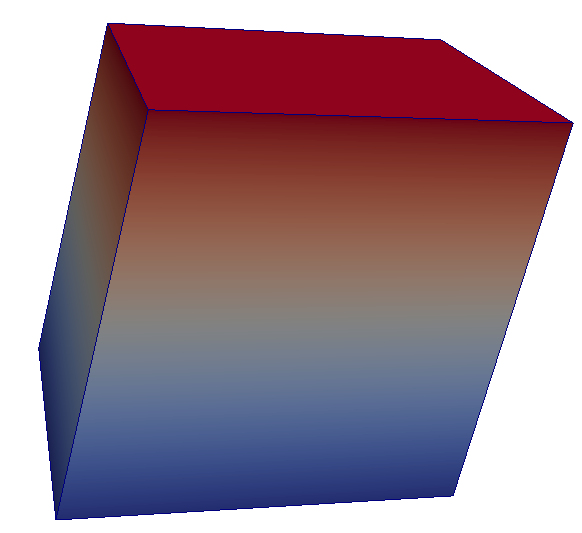
\includegraphics[width = 3cm]{./Figure-files/Day3/Single_element_Models_illustrate_the_elastic-plastic_behavior/overview.png}
  \caption{Simulation Model of Single Element}
  \label{fig_single_element_elastic_plastic_vmGGmax}
\end{figure}



\begin{figure*}[!htbp]
    \centering
    \begin{subfigure}[b]{0.475\textwidth}
        \centering
        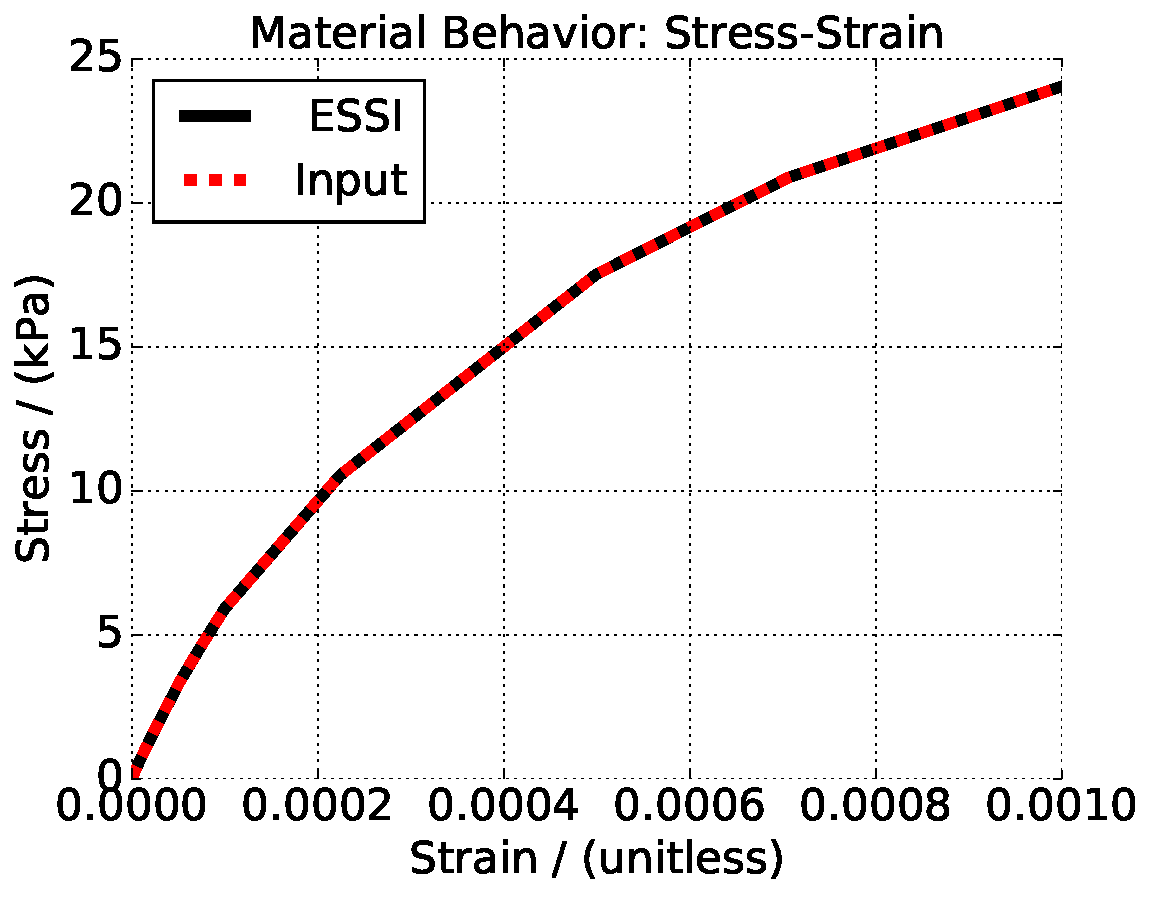
\includegraphics[width=\textwidth]{./Figure-files/Day3/Single_element_Models_illustrate_the_elastic-plastic_behavior/vmGGmax/1/backbone.pdf}
        \caption[]%
        {{\small Stress-Strain Curves}}    
    \end{subfigure}
    \hfill
    \begin{subfigure}[b]{0.475\textwidth}  
        \centering 
        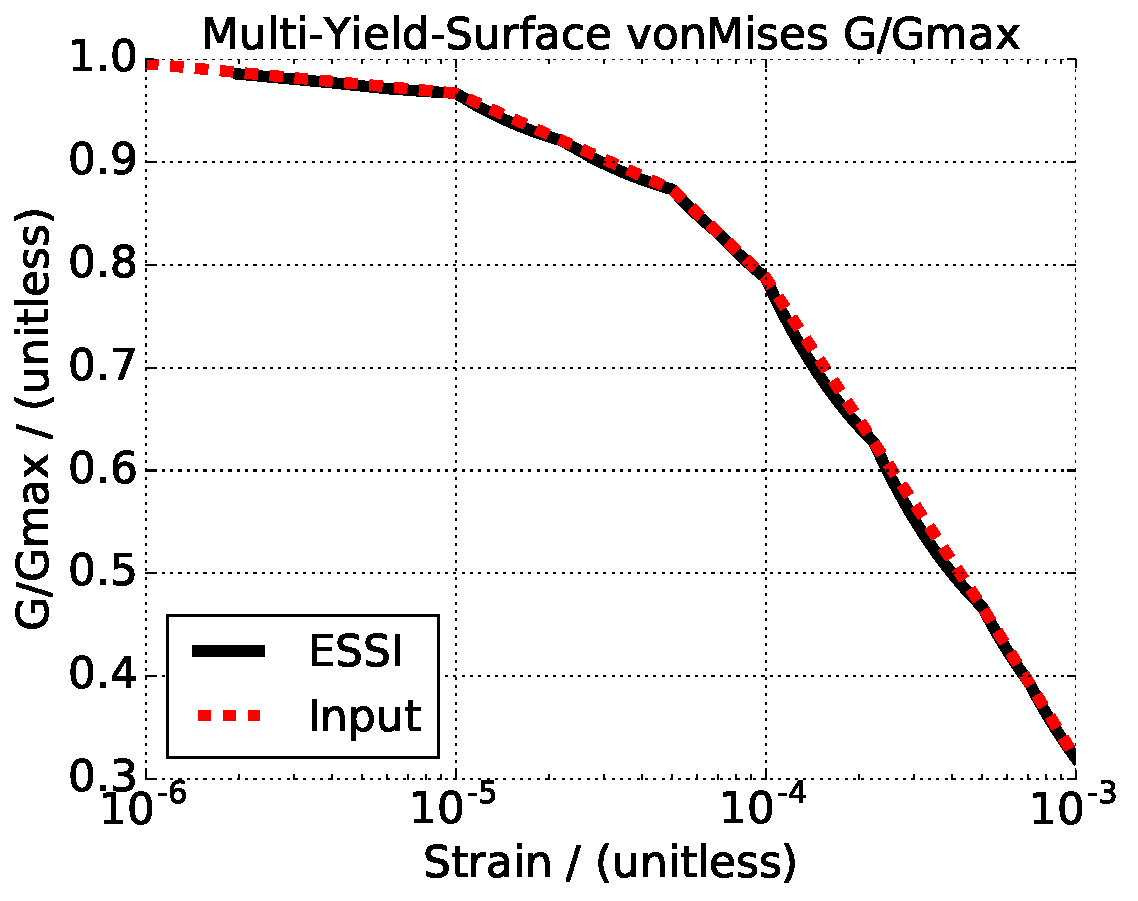
\includegraphics[width=\textwidth]{./Figure-files/Day3/Single_element_Models_illustrate_the_elastic-plastic_behavior/vmGGmax/1/GGmax.pdf}
        \caption[]%
        {{\small G/Gmax Comparison}}    
    \end{subfigure}
    \vskip\baselineskip
    \begin{subfigure}[b]{0.475\textwidth}   
        \centering 
        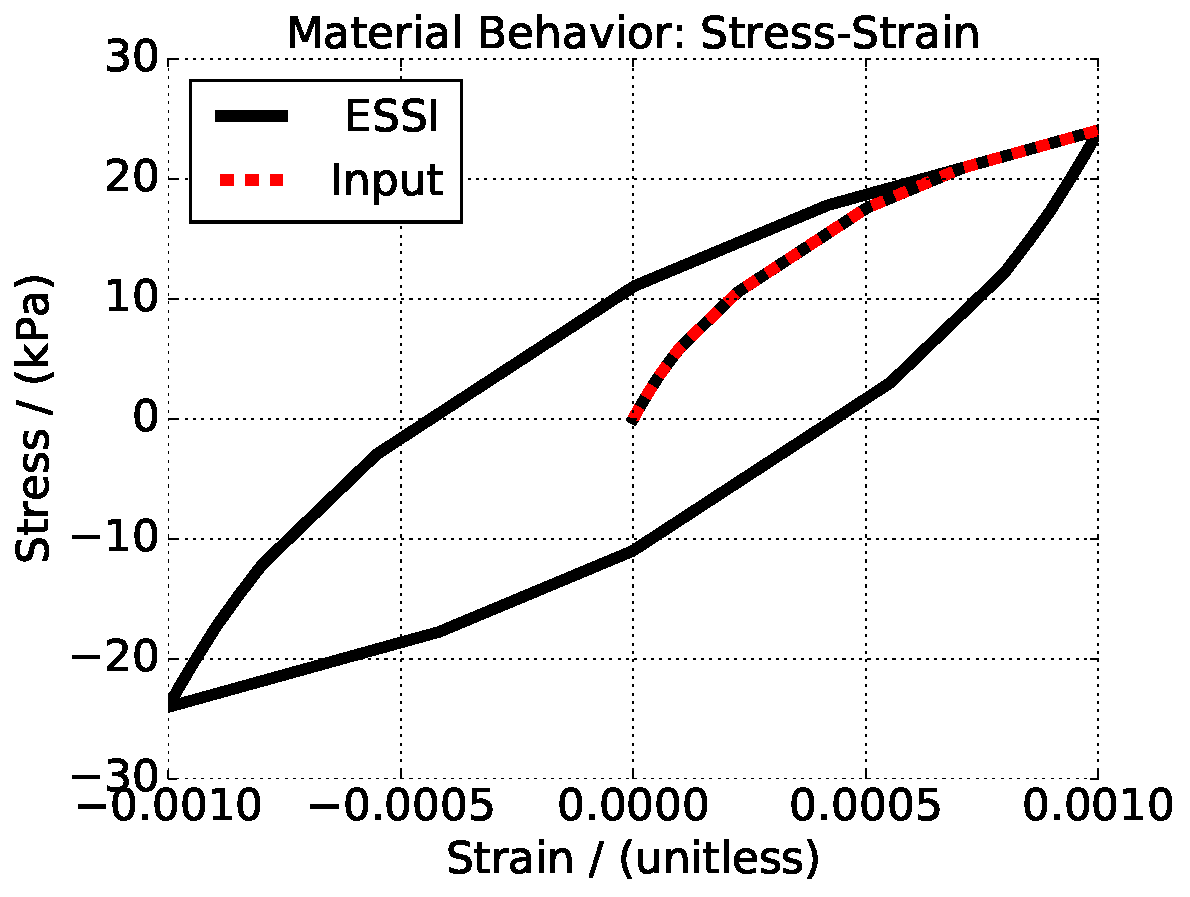
\includegraphics[width=\textwidth]{./Figure-files/Day3/Single_element_Models_illustrate_the_elastic-plastic_behavior/vmGGmax/1/full-loop.pdf}
        \caption[]%
        {{\small One Cyclic Stress-Strain Curves}}    
    \end{subfigure}
    \quad
    \begin{subfigure}[b]{0.475\textwidth}   
        \centering 
        \includegraphics[width=\textwidth]{./Figure-files/Day3/Single_element_Models_illustrate_the_elastic-plastic_behavior/vmGGmax/1/damping.pdf}
        \caption[]%
        {{\small Damping Plot Curves}}    
    \end{subfigure}
    \caption[ Multi-Yield-Surface von-Mises]
    {\small Multi-Yield-Surface von-Mises} 
    \label{fig_Multi-Yield-Surface_von-Mises}
\end{figure*}




% ******************************************************************
% ******************************************************************
% ******************************************************************
\clearpage
\newpage
\subsection{Drucker-Prager perfectly plastic material model}

\paragraph{Drucker-Prager perfectly plastic material model}

The Real-ESSI input files for this Drucker-Prager perfectly plastic example are available 
\href{http://cml01.engr.ucdavis.edu/shortCourse/Day3/Single_element_Models_illustrate_the_elastic-plastic_behavior/DPpp}{HERE}. 
The compressed package of Real-ESSI input files for this example is available 
\href{http://cml01.engr.ucdavis.edu/shortCourse/Day3/Single_element_Models_illustrate_the_elastic-plastic_behavior/DPpp/DPpp.tgz}{HERE}. 


\paragraph{Drucker-Prager Armstrong-Frederick Non-associate material model}

The Real-ESSI input files for this Drucker-Prager Armstrong-Frederick example are available 
\href{http://cml01.engr.ucdavis.edu/shortCourse/Day3/Single_element_Models_illustrate_the_elastic-plastic_behavior/DPaf}{HERE}. 
The compressed package of Real-ESSI input files for this example is available 
\href{http://cml01.engr.ucdavis.edu/shortCourse/Day3/Single_element_Models_illustrate_the_elastic-plastic_behavior/DPaf/DPaf.tgz}{HERE}. 





\begin{figure}[H]
  \centering
  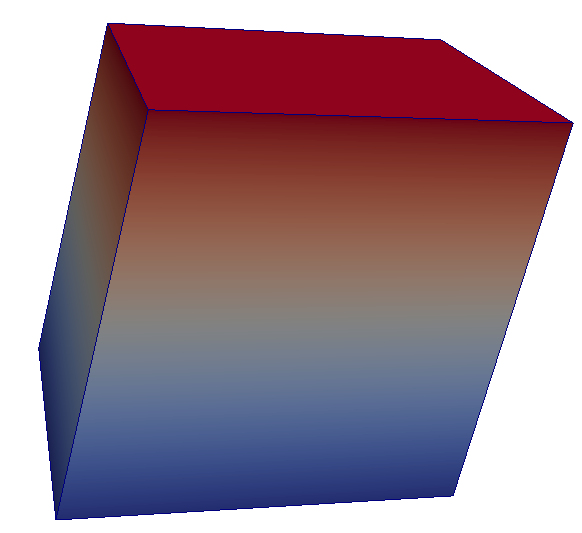
\includegraphics[width = 6cm]{./Figure-files/Day3/Single_element_Models_illustrate_the_elastic-plastic_behavior/overview.png}
  \caption{Simulation Model of Single Element}
  \label{fig_single_element_elastic_plastic2}
\end{figure}


The illustration results are shown in Fig.~\ref{fig_single_element_elastic_plastic_dppp_dpaf}.

\begin{figure}[H]
  \centering
  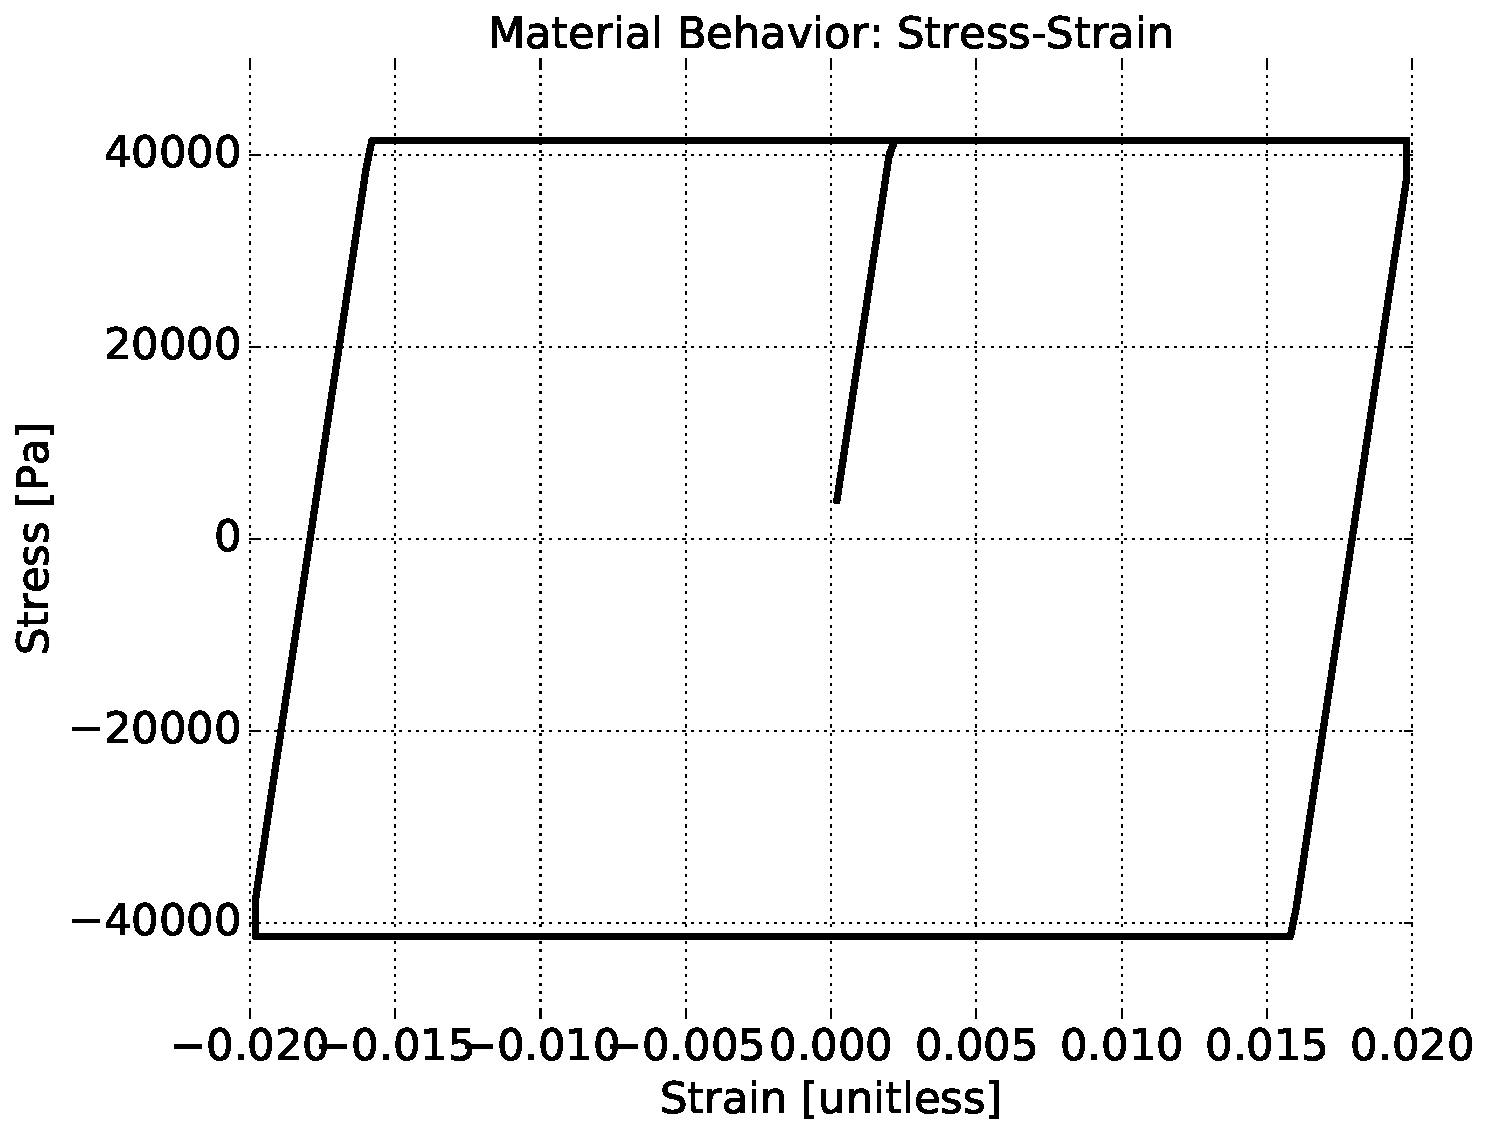
\includegraphics[width = 7cm]{./Figure-files/Day3/Single_element_Models_illustrate_the_elastic-plastic_behavior/dppp.pdf}
  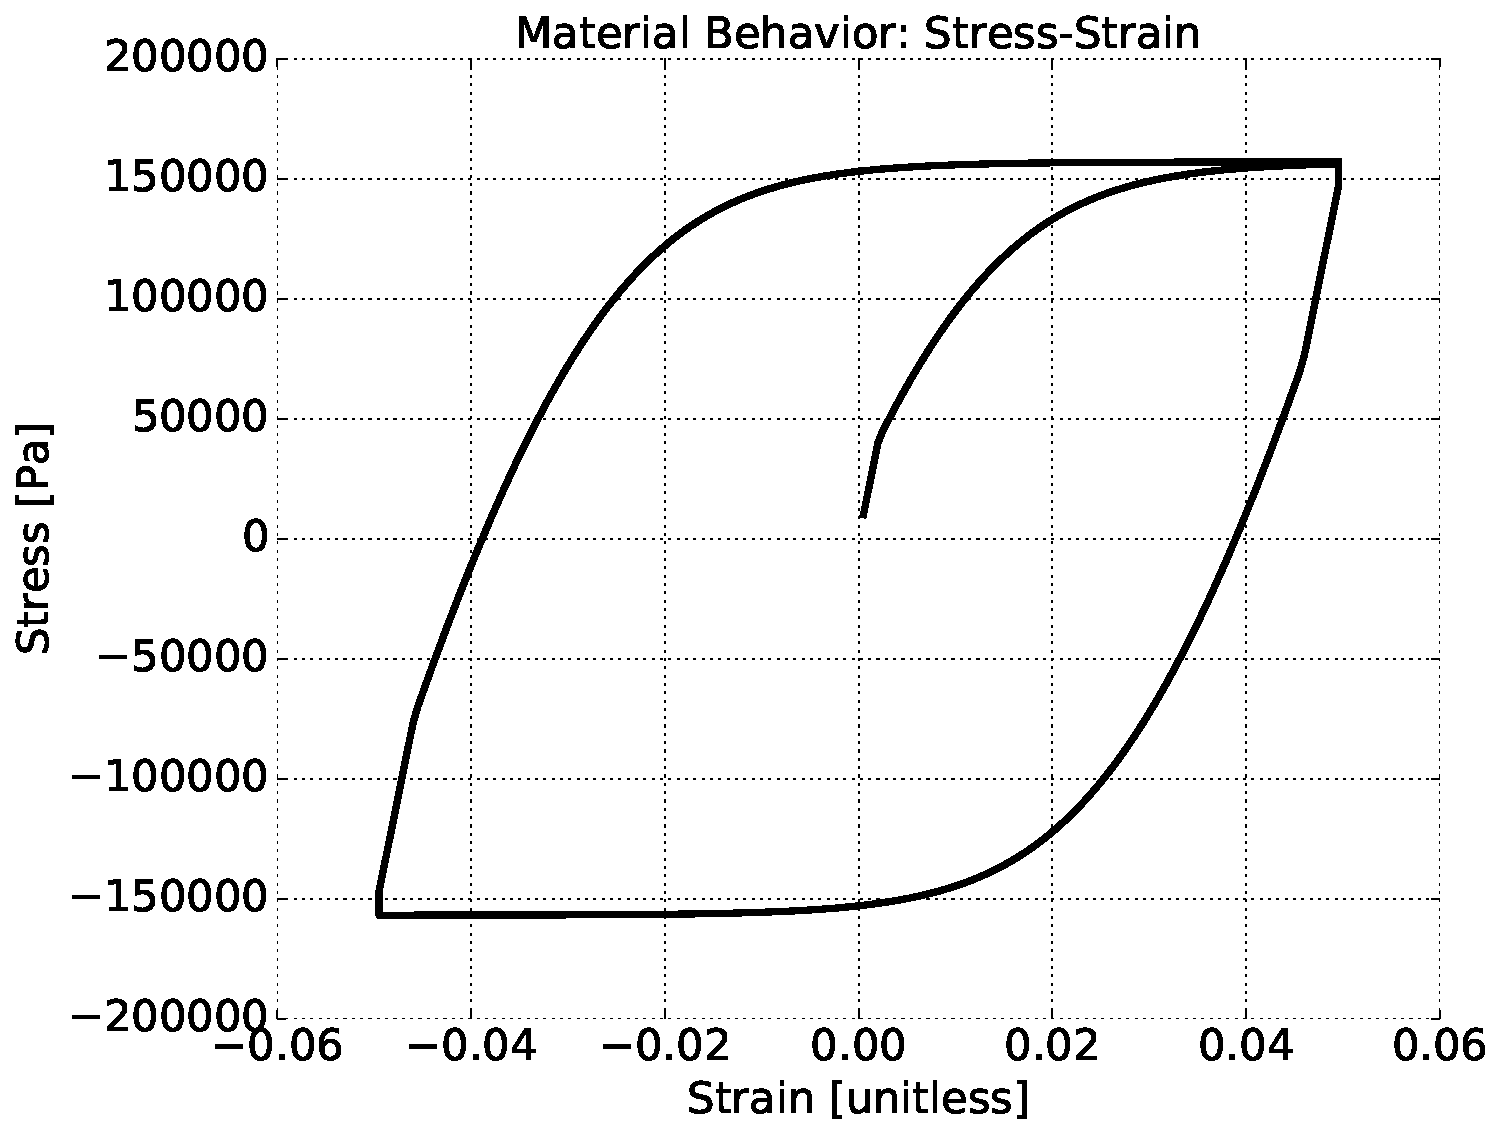
\includegraphics[width = 7cm]{./Figure-files/Day3/Single_element_Models_illustrate_the_elastic-plastic_behavior/dpaf.pdf}
  \caption{Simulation Results of Single Element}
  \label{fig_single_element_elastic_plastic_dppp_dpaf}
\end{figure}




% ******************************************************************
% ******************************************************************
% ******************************************************************
\clearpage
\newpage
\subsection{Drucker-Prager G/Gmax Non-associate material model}



The Real-ESSI input files for this example are available 
\href{http://cml01.engr.ucdavis.edu/shortCourse/Day3/Single_element_Models_illustrate_the_elastic-plastic_behavior/DPGGmax}{HERE}. 
The compressed package of Real-ESSI input files for this example is available 
\href{http://cml01.engr.ucdavis.edu/shortCourse/Day3/Single_element_Models_illustrate_the_elastic-plastic_behavior/DPGGmax/DPGGmax.tgz}{HERE}. 

The Modeling parameters are listed.
\begin{itemize}
  \item Drucker-Prager G/Gmax material model 
  \begin{itemize}
    \item Mass density, $\rho$, \enspace \enspace 2000 $kg/m^3$
    \item Young's modulus, $E$, \enspace \enspace 200 MPa
    \item Poisson's ratio, $\nu$, \enspace \enspace 0.1
    \item Initial confining stress, $p_0$, \enspace \enspace 100 kPa
    \item Reference pressure, $p_{refer} $, \enspace \enspace 100 kPa
    \item Pressure exponential, $ n  $, \enspace \enspace 0.5
    \item Cohesion, $ n  $, \enspace \enspace 1 kPa
    \item Total number of Shear Modulus \enspace \enspace 9
    \item G over Gmax, \enspace \enspace  1,0.995,0.966,0.873,0.787,0.467,0.320,0.109,0.063
    \item Shear strain gamma, \enspace \enspace  0,1E-6,1E-5,5E-5,1E-4, 0.0005, 0.001, 0.005, 0.01
  \end{itemize}
\end{itemize}

\begin{figure}[H]
  \centering
  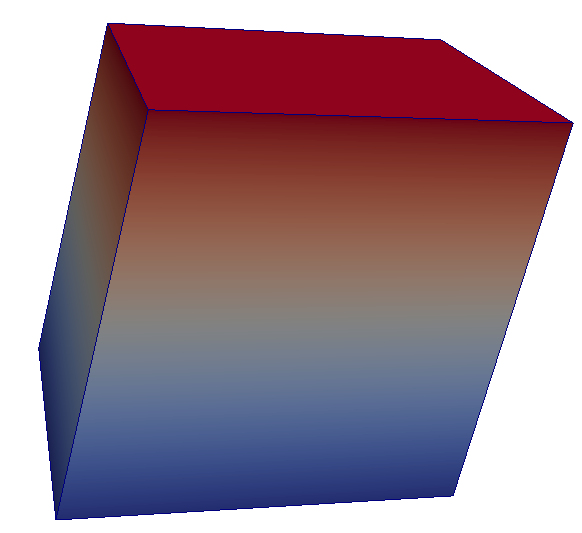
\includegraphics[width = 6cm]{./Figure-files/Day3/Single_element_Models_illustrate_the_elastic-plastic_behavior/overview.png}
  \caption{Simulation Model of Single Element}
  \label{fig_single_element_elastic_plastic3}
\end{figure}


The illustration results are shown in Fig.~\ref{fig_single_element_elastic_plastic_dpGGmax}.

\begin{figure}[H]
  \centering
  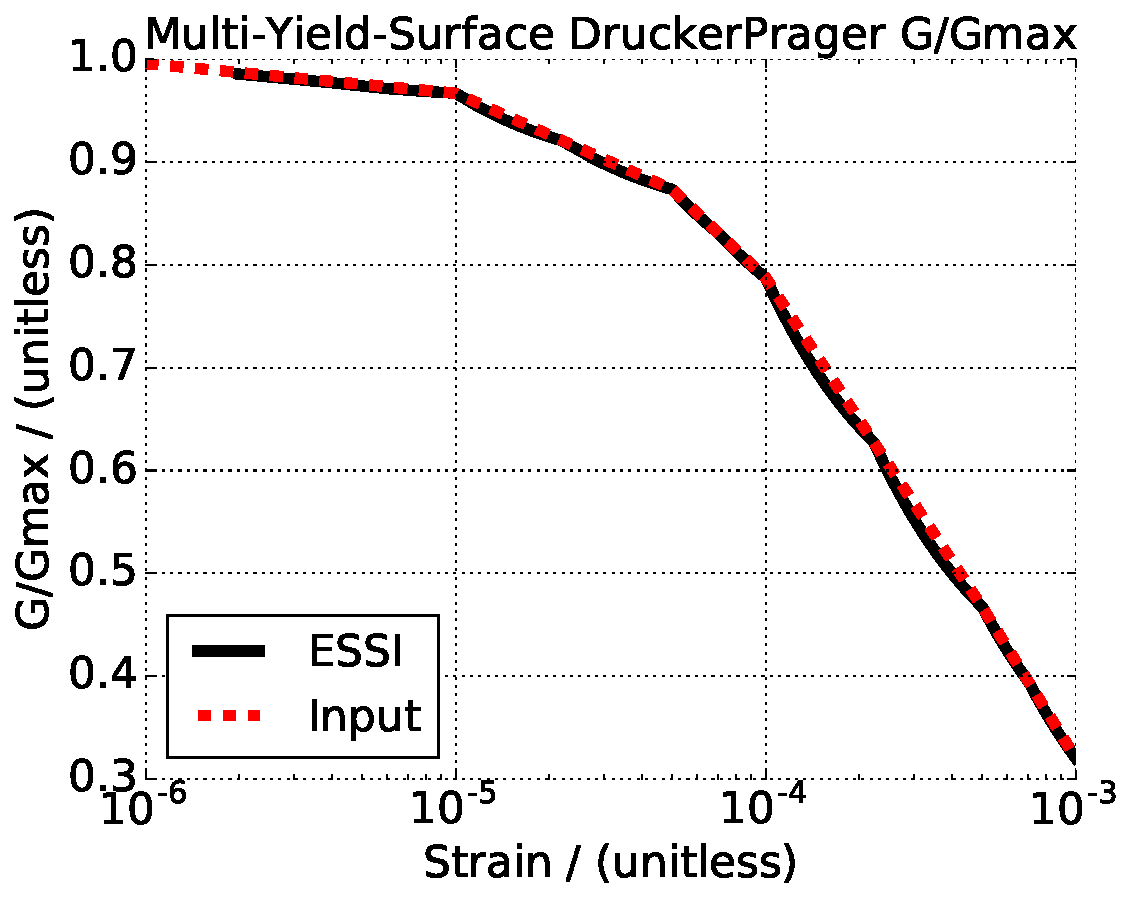
\includegraphics[width = 7cm]{./Figure-files/Day3/Single_element_Models_illustrate_the_elastic-plastic_behavior/dpGGmax/1/GGmax.pdf}
  \includegraphics[width = 7cm]{./Figure-files/Day3/Single_element_Models_illustrate_the_elastic-plastic_behavior/dpGGmax/1/damping.pdf}
  \caption{Simulation Results of Single Element}
  \label{fig_single_element_elastic_plastic_dpGGmax}
\end{figure}



% ******************************************************************
% ******************************************************************
% ******************************************************************
\clearpage
\newpage
\section{Wave Propagation through elastoplastic Soil}
\label{Wave_Propagation_through_elastoplastic_Soil}


The Real-ESSI input files for this example are available 
\href{http://cml01.engr.ucdavis.edu/shortCourse/Day3/Wave_Propagation_through_elastoplastic_Soil}{HERE}. 
The compressed package of Real-ESSI input files for this example is available 
\href{http://cml01.engr.ucdavis.edu/shortCourse/Day3/Wave_Propagation_through_elastoplastic_Soil/Wave_Propagation_through_elastoplastic_Soil.tgz}{HERE}. 

\begin{figure}[H]
  \centering
  \includegraphics[width = 0.6cm]{./Figure-files/Day3/Wave_Propagation_through_elastoplastic_Soil/overview.png}
  \caption{Wave Propagation through elastoplastic Soils}
  \label{fig_wave_propagation_elastoplastic}
\end{figure}


The displacement series at the surface are plotted in time and frequency domain.


\begin{figure}[H]
  \centering
  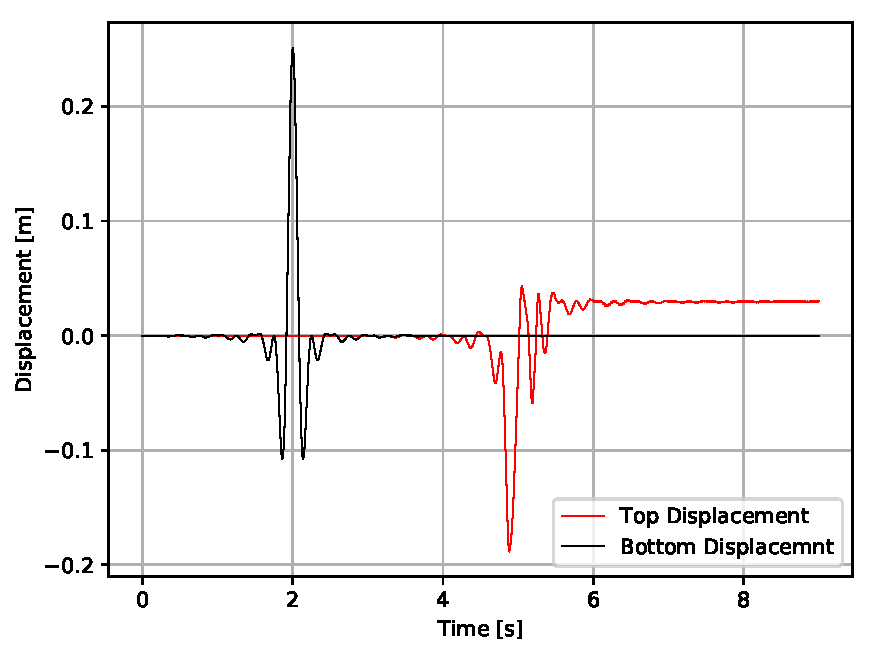
\includegraphics[width = 8cm]{./Figure-files/Day3/Wave_Propagation_through_elastoplastic_Soil/Displacement.pdf}
  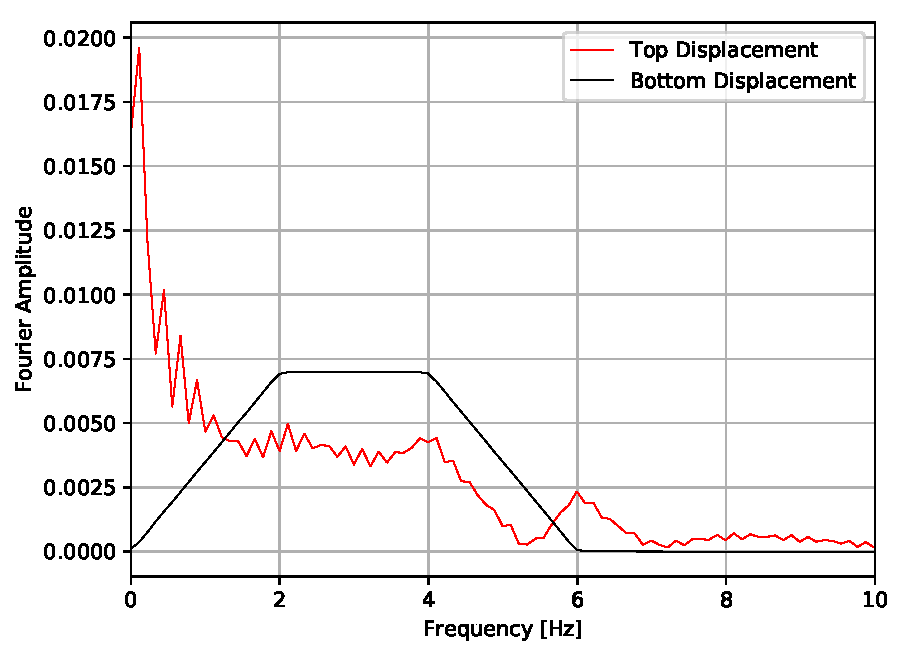
\includegraphics[width = 8cm]{./Figure-files/Day3/Wave_Propagation_through_elastoplastic_Soil/Displacement_Spectrum.pdf}
  \caption{Simulation Results of Wave Propagation}
  \label{fig_elastic_plastic_wave_propagation}
\end{figure}


% \paragraph{Another Set of Solution with motion reduction}

% The displacement series with motion reduction are plotted in time and frequency domain.

% \begin{figure}[H]
%   \centering
%   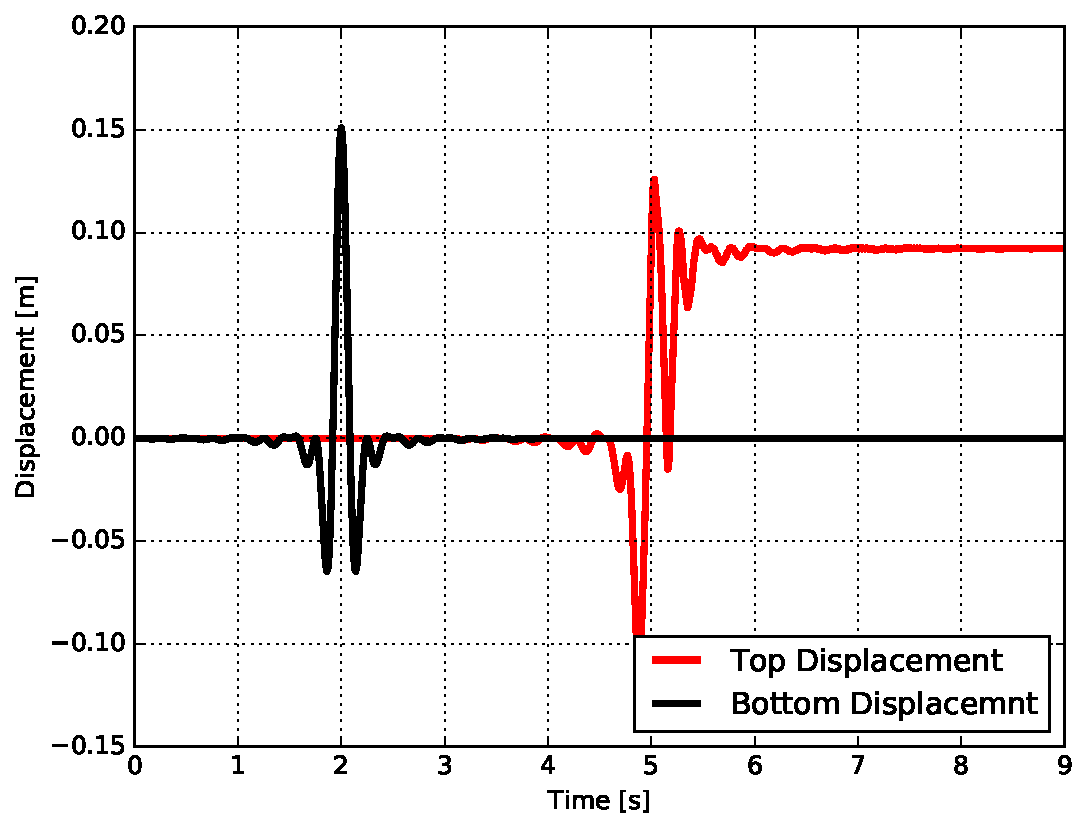
\includegraphics[width = 8cm]{./Figure-files/Day3/Wave_Propagation_through_elastoplastic_Soil/2Displacement.pdf}
%   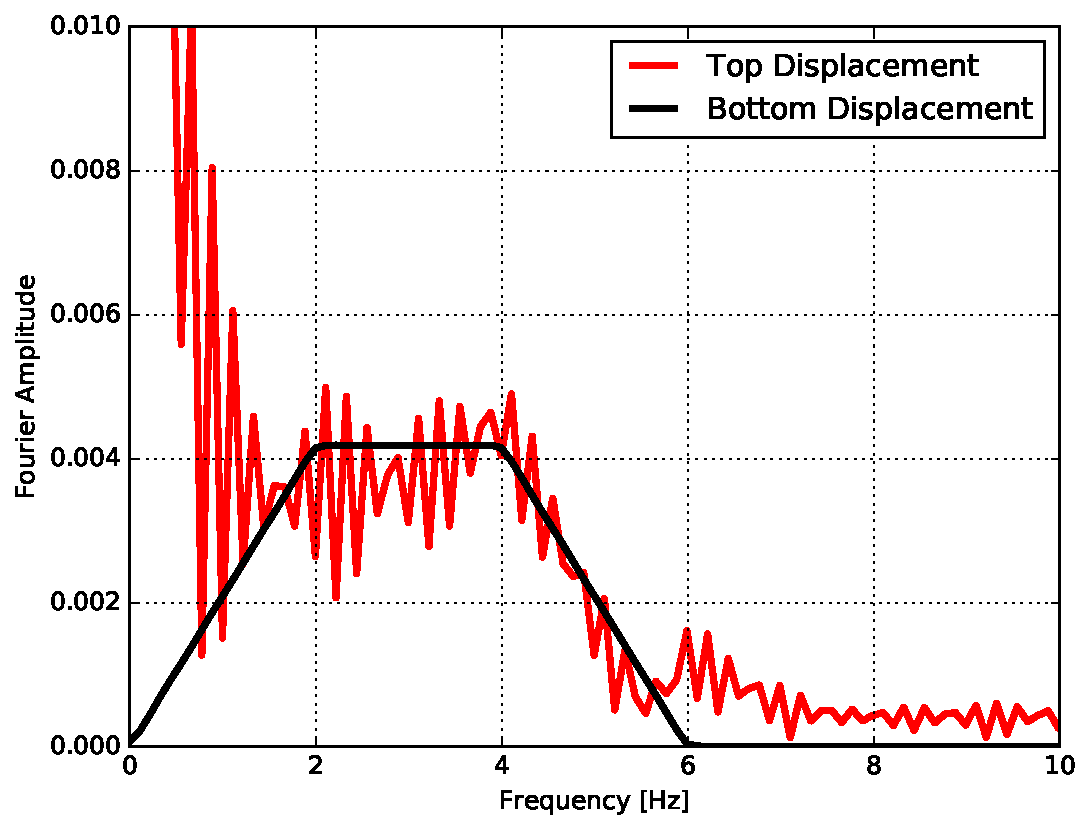
\includegraphics[width = 8cm]{./Figure-files/Day3/Wave_Propagation_through_elastoplastic_Soil/2Displacement_Spectrum.pdf}
%   \caption{Simulation Results of Wave Propagation (motion reduction)}
%   \label{fig_elastic_plastic_wave_propagation_Half}
% \end{figure}






% ******************************************************************
% ******************************************************************
% ******************************************************************
\clearpage
\newpage
\section{Contact Examples}
\label{Contact_Examples}
\subsection{ Axial behavior: Stress Based Contact Element}


\paragraph{Stress-Based Hard Contact Example}
The Real-ESSI input files for hard contact example are available 
\href{http://cml01.engr.ucdavis.edu/shortCourse/Day3/Contact_Examples/axial/HardContact_Elastic_Perfectly_Plastic_Shear_Model}{HERE}. 
The compressed package of Real-ESSI input files for this example is available 
\href{http://cml01.engr.ucdavis.edu/shortCourse/Day3/Contact_Examples/axial/HardContact_Elastic_Perfectly_Plastic_Shear_Model/HardContact_Elastic_Perfectly_Plastic_Shear_Model.tgz}{HERE}. 

\paragraph{Stress-Based Soft Contact Example}
The Real-ESSI input files for soft contact example are available 
\href{http://cml01.engr.ucdavis.edu/shortCourse/Day3/Contact_Examples/axial/SoftContact_Elastic_Perfectly_Plastic_Shear_Model}{HERE}. 
The compressed package of Real-ESSI input files for this example is available 
\href{http://cml01.engr.ucdavis.edu/shortCourse/Day3/Contact_Examples/axial/SoftContact_Elastic_Perfectly_Plastic_Shear_Model/SoftContact_Elastic_Perfectly_Plastic_Shear_Model.tgz}{HERE}. 


The axial behavior of hard contact and soft contact are illustrated in Fig.~\ref{fig_soft_hard_contact}.



\begin{figure}[H]
  \centering
  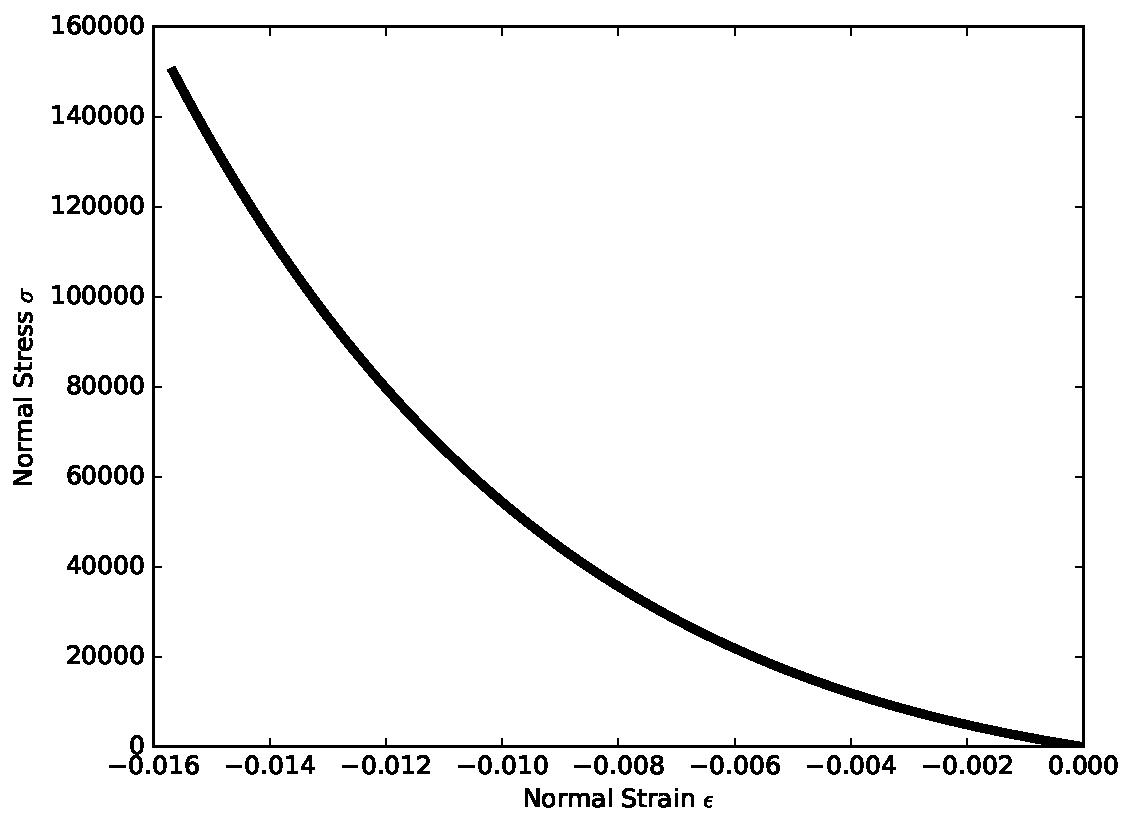
\includegraphics[width = 8cm]{./Figure-files/Day3/Contact_Examples/softcontact.pdf}
  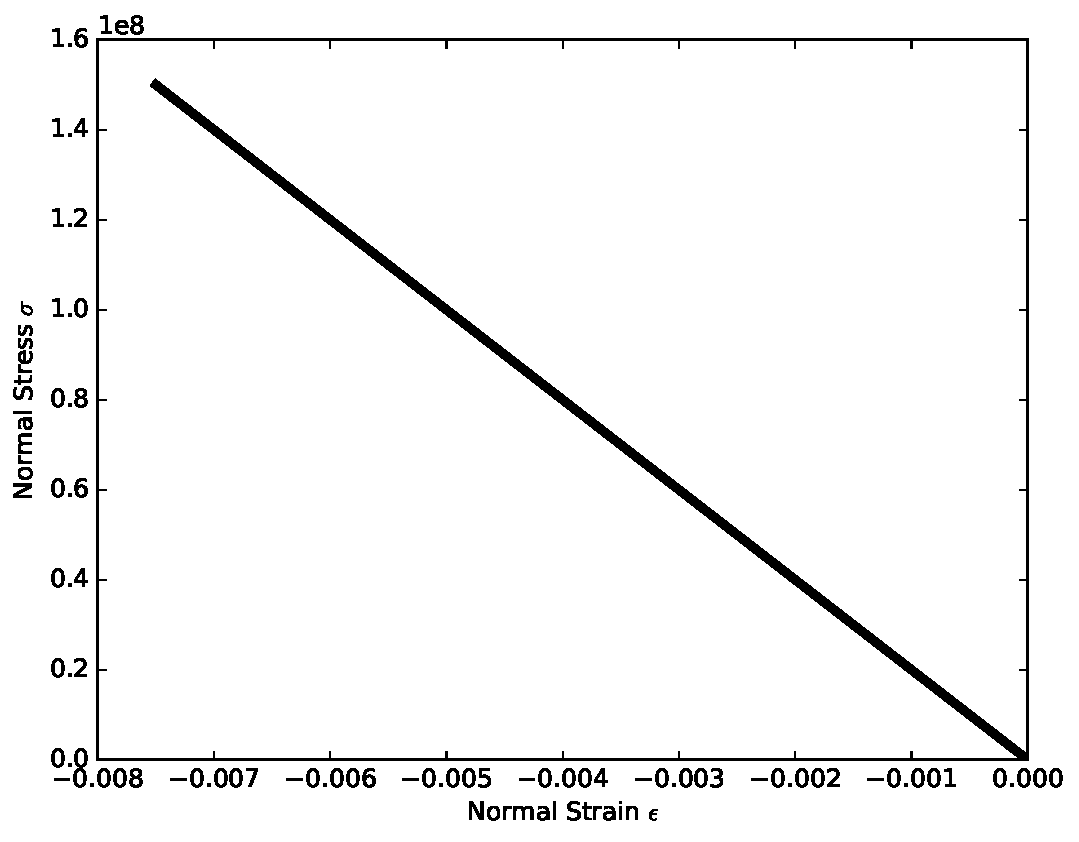
\includegraphics[width = 8cm]{./Figure-files/Day3/Contact_Examples/hardcontact.pdf}
  \caption{Simulation Results of Soft Contact and Hard Contact}
  \label{fig_soft_hard_contact}
\end{figure}






% ******************************************************************
% ******************************************************************
% ******************************************************************
\clearpage
\newpage
\subsection{ Shear behavior: Stress Based Contact }


\paragraph{Stress-Based Elastic-perfectly plastic contact}
The Real-ESSI input files for the the elastic-perfectly plastic example are available 
\href{http://cml01.engr.ucdavis.edu/shortCourse/Day3/Contact_Examples/shear/SoftContact_Elastic_Perfectly_Plastic_Shear_Model}{HERE}. 
The compressed package of Real-ESSI input files for this example is available 
\href{http://cml01.engr.ucdavis.edu/shortCourse/Day3/Contact_Examples/shear/SoftContact_Elastic_Perfectly_Plastic_Shear_Model/SoftContact_Elastic_Perfectly_Plastic_Shear_Model.tgz}{HERE}. 


\paragraph{Stress-Based Elastic-hardening contact}

The Real-ESSI input files for the elastic-hardening contact example are available 
\href{http://cml01.engr.ucdavis.edu/shortCourse/Day3/Contact_Examples/shear/SoftContact_Nonlinear_Hardening_Shear_Model}{HERE}. 
The compressed package of Real-ESSI input files for this example is available 
\href{http://cml01.engr.ucdavis.edu/shortCourse/Day3/Contact_Examples/shear/SoftContact_Nonlinear_Hardening_Shear_Model/SoftContact_Nonlinear_Hardening_Shear_Model.tgz}{HERE}. 



\paragraph{Stress-Based Elastic-hardening-softening contact}

The Real-ESSI input files for the elastic-hardening-softening example are available 
\href{http://cml01.engr.ucdavis.edu/shortCourse/Day3/Contact_Examples/shear/SoftContact_Nonlinear_Hardening_Softening_Shear_Model}{HERE}. 
The compressed package of Real-ESSI input files for this example is available 
\href{http://cml01.engr.ucdavis.edu/shortCourse/Day3/Contact_Examples/shear/SoftContact_Nonlinear_Hardening_Softening_Shear_Model/SoftContact_Nonlinear_Hardening_Softening_Shear_Model.tgz}{HERE}. 



The axial behavior of hard contact and soft contact are illustrated in Fig.~\ref{fig_soft_hard_contact_shear}.


\begin{figure}[H]
  \centering
  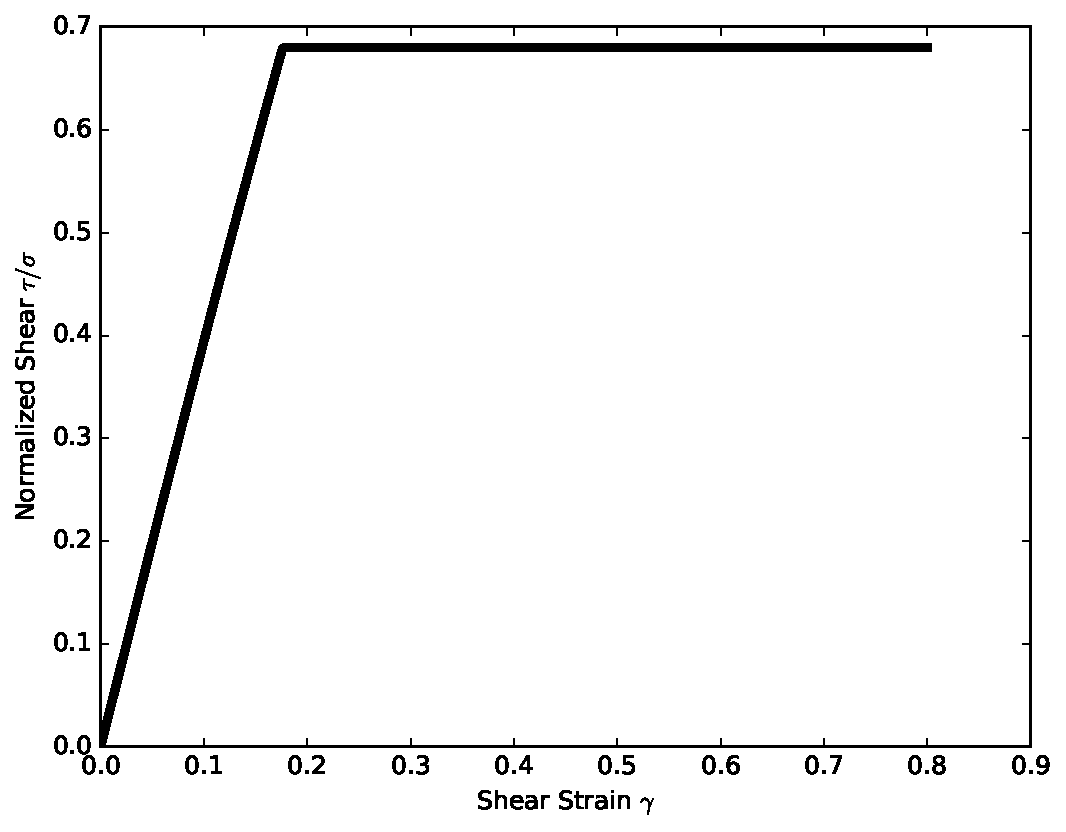
\includegraphics[width = 8cm]{./Figure-files/Day3/Contact_Examples/shear_perfectly_plastic.pdf}
  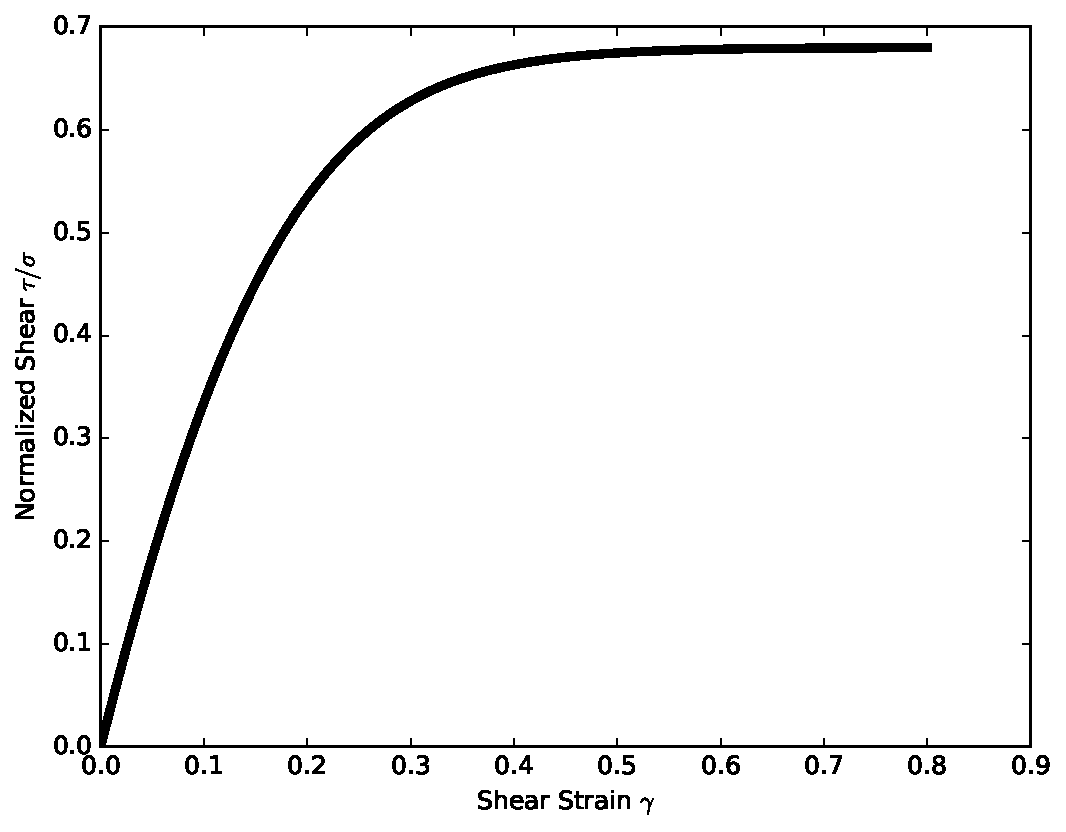
\includegraphics[width = 8cm]{./Figure-files/Day3/Contact_Examples/shear_hard.pdf}
  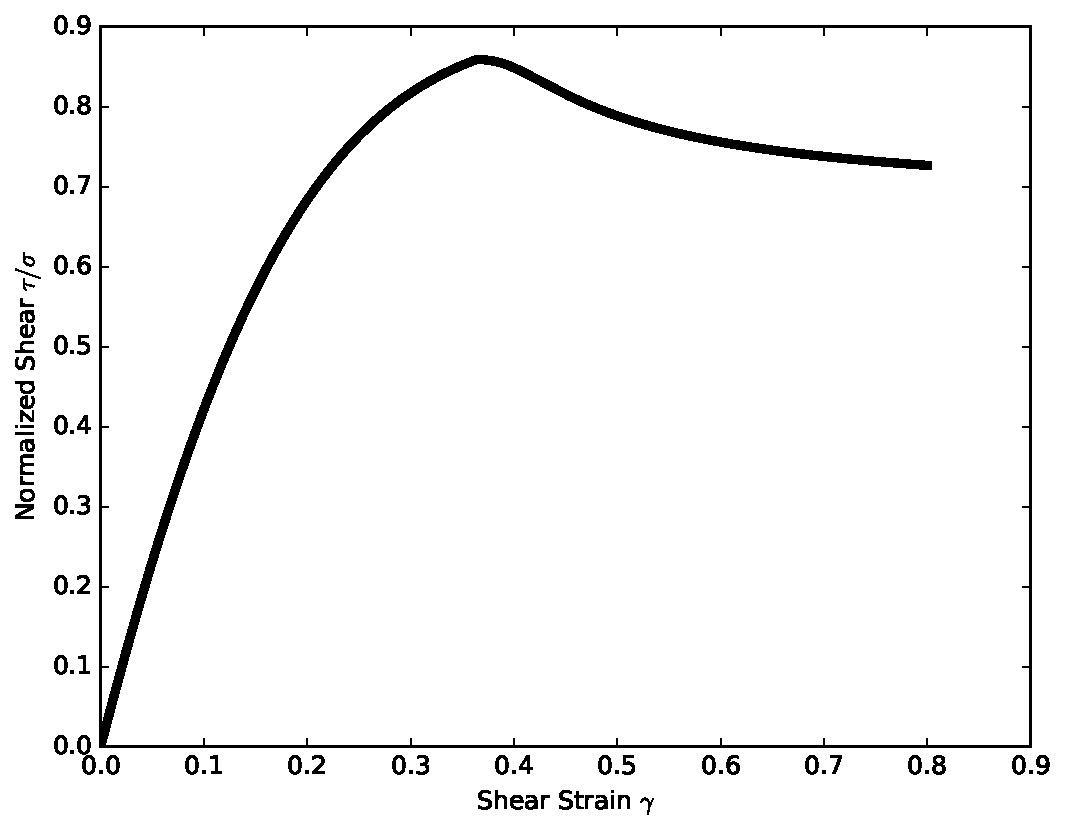
\includegraphics[width = 8cm]{./Figure-files/Day3/Contact_Examples/shear_hard_soft.pdf}
  \caption{Simulation Results of Shear Bahaviors in Stress Based Contact Elements}
  \label{fig_soft_hard_contact_shear}
\end{figure}






% ******************************************************************
% ******************************************************************
% ******************************************************************
\clearpage
\newpage
\subsection{ Force Based Contact Example: Base Isolator}

The Real-ESSI input files for this example are available 
\href{http://cml01.engr.ucdavis.edu/shortCourse/Day3/Contact_Examples/force_based}{HERE}. 
The compressed package of Real-ESSI input files for this example is available 
\href{http://cml01.engr.ucdavis.edu/shortCourse/Day3/Contact_Examples/force_based/force_based.tgz}{HERE}. 


\begin{figure}[H]
  \centering
  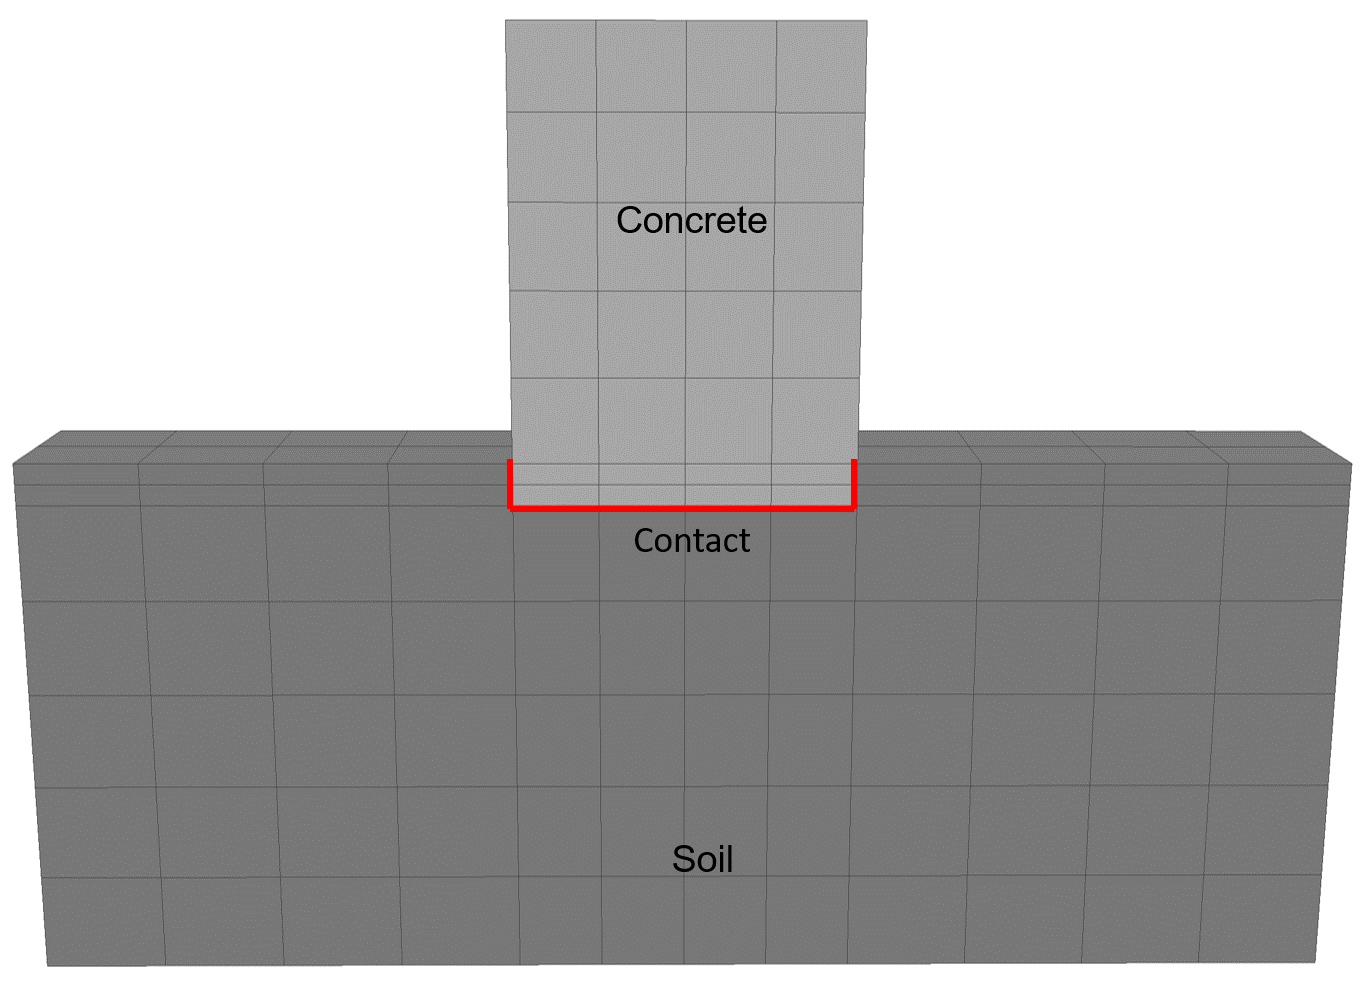
\includegraphics[width = 8cm]{./Figure-files/Day3/Contact_Examples/Model_Description.png}
  \caption{Simulation Model}
  \label{fig_contact_examples_base_isolator}
\end{figure}

The illustration results are show in Fig.\ref{fig_contact_examples_base_isolator_results}.


\begin{figure}[H]
  \centering
  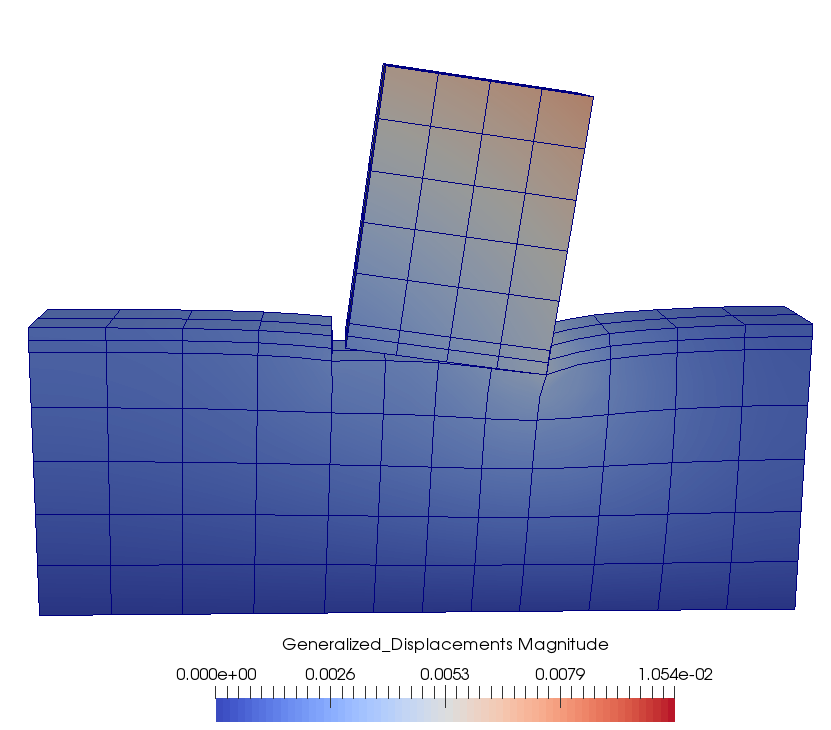
\includegraphics[width = 8cm]{./Figure-files/Day3/Contact_Examples/Uniform_Acceleration_0_85_sec.png}
  \caption{Simulation Results of Contact Examples}
  \label{fig_contact_examples_base_isolator_results}
\end{figure}






% ******************************************************************
% ******************************************************************
% ******************************************************************
\clearpage
\newpage
\section{ Frame Pushover}
\label{Frame_Pushover}


The Real-ESSI input files for this example are available 
\href{http://cml01.engr.ucdavis.edu/shortCourse/Day3/Frame_Pushover}{HERE}. 
The compressed package of Real-ESSI input files for this example is available 
\href{http://cml01.engr.ucdavis.edu/shortCourse/Day3/Frame_Pushover/Frame_Pushover.tgz}{HERE}. 


The Modeling parameters are listed.
\begin{itemize}
  \item Uniaxial concrete 
  \begin{itemize}
    \item Compressive strength,  \enspace \enspace 24 MPa
    \item Strain at compressive strength,  \enspace \enspace 0.001752
    \item Crushing strength,  \enspace \enspace 0.0 Pa
    \item Strain at compressive strength,  \enspace \enspace 0.003168
    \item lambda, \enspace \enspace 0.5
    \item Tensile strength, \enspace \enspace 0 Pa
    \item Tension softening stiffness, \enspace \enspace 0 Pa
  \end{itemize}
  \item Uniaxial steel
  \begin{itemize}
    \item Yield strength, \enspace \enspace 413.8 MPa
    \item Young's modulus, \enspace \enspace 200 GPa
    \item Strain hardening ratio, \enspace \enspace 0.01
    \item R0, \enspace \enspace 18.0
    \item cR1,  \enspace \enspace 0.925
    \item cR2,  \enspace \enspace 0.15
    \item a1, \enspace \enspace 0.0
    \item a2, \enspace \enspace 55.0
    \item a3, \enspace \enspace 0.0
    \item a4, \enspace \enspace 55.0
  \end{itemize}
\end{itemize}



\begin{figure}[H]
  \centering
  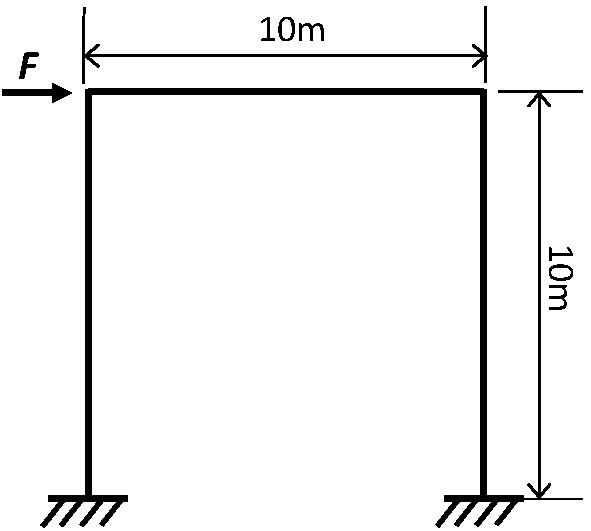
\includegraphics[width = 7cm]{./Figure-files/Day3/Frame_Pushover/overview.pdf}
  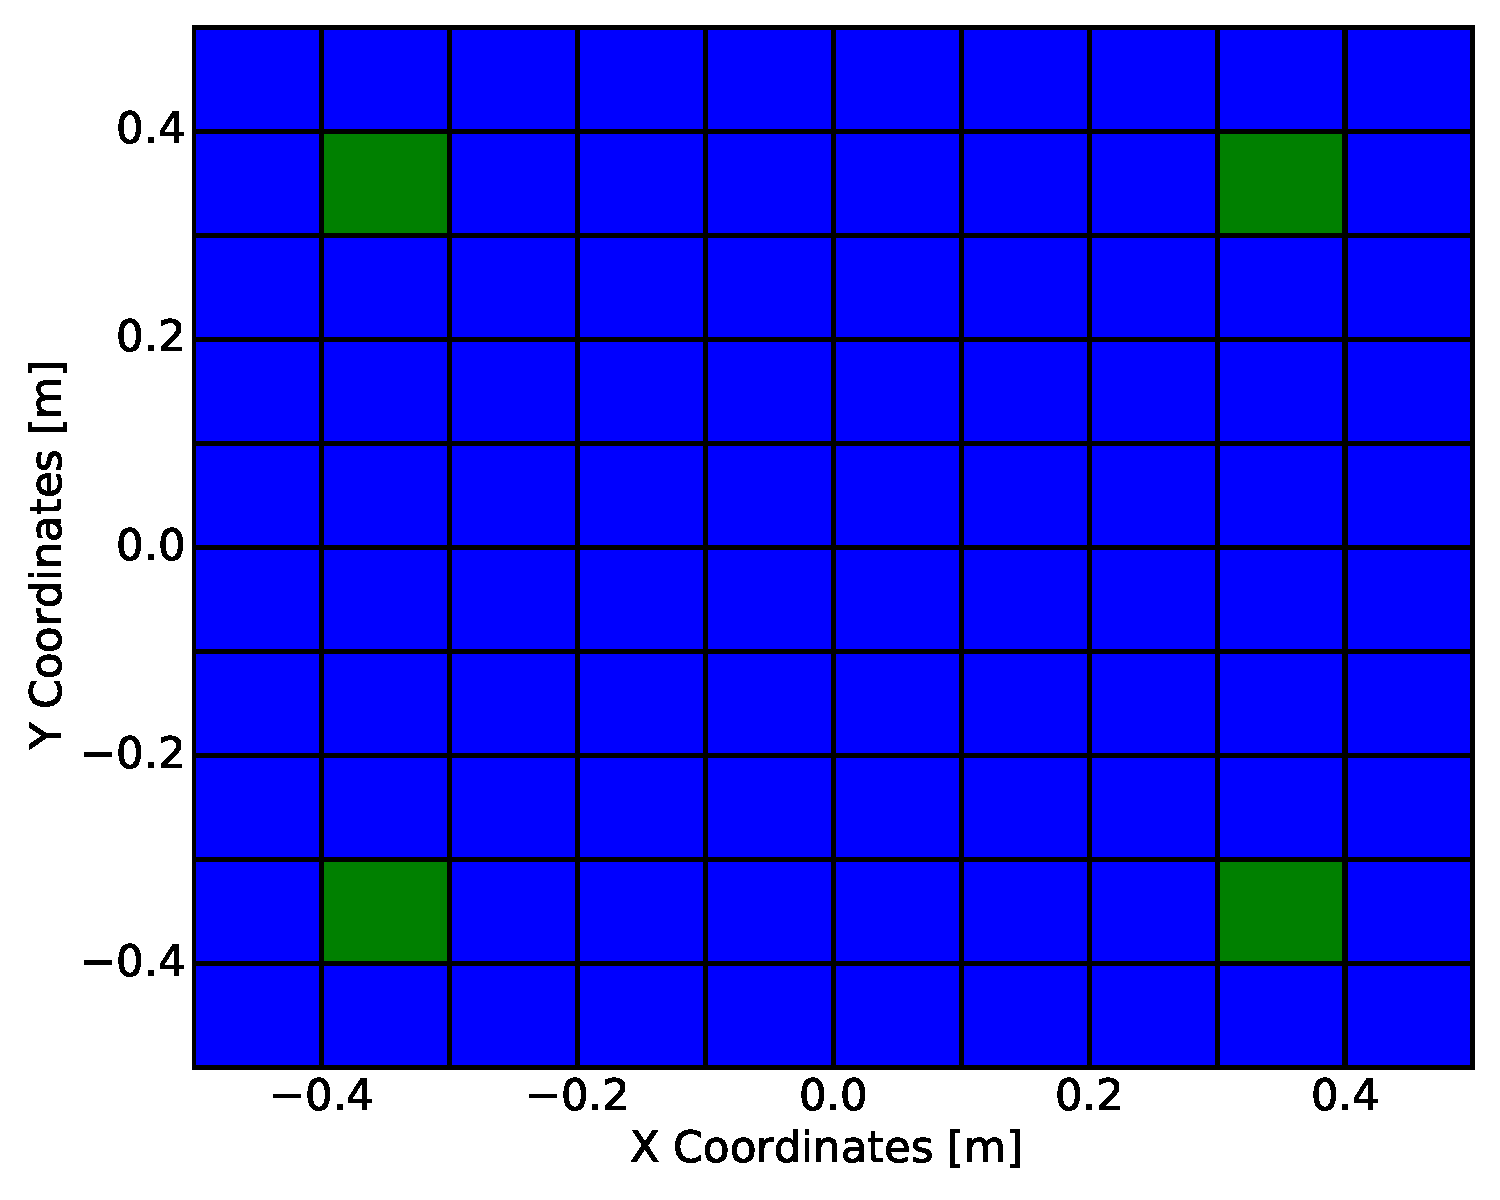
\includegraphics[width = 7cm]{./Figure-files/Day3/Frame_Pushover/rectangle_rebar2.pdf}
  \caption{Model of Pushover Simulation and the Cross Section of Fiber Beam (Concrete and Rebar) }
  \label{fig_frame_pushover}
\end{figure}

The illustrative result is shown in Fig.~\ref{fig_day3_fiberbeam_pushover_results}.

\begin{figure}[H]
  \centering
  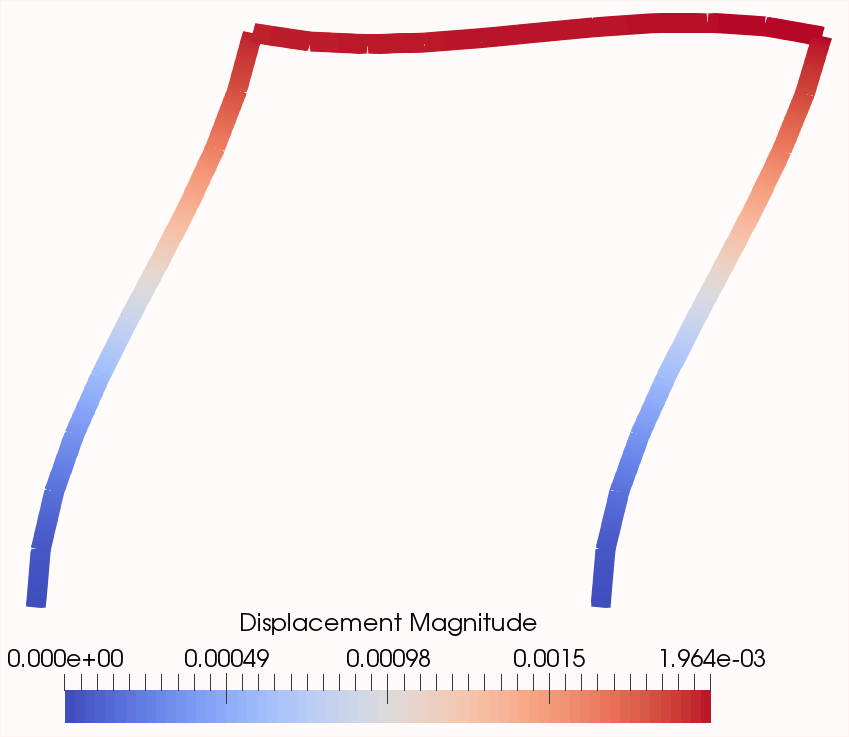
\includegraphics[width = 8cm]{./Figure-files/Day3/Frame_Pushover/fiberBeamDeform.png}
  \caption{Illustration results of Fiber Pushover}
  \label{fig_day3_fiberbeam_pushover_results}
\end{figure}

\begin{figure}[H]
  \centering
  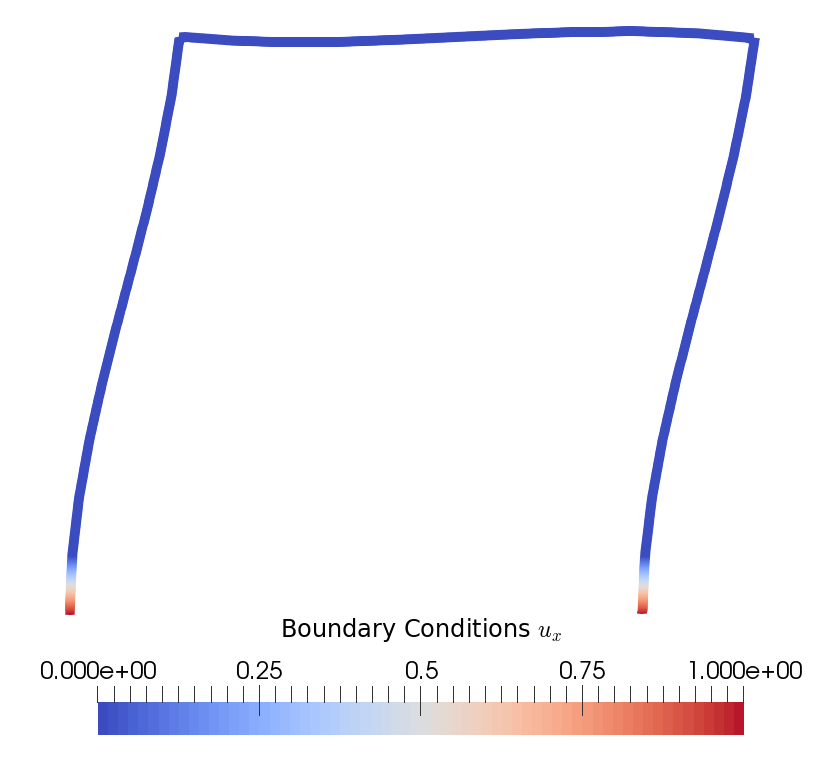
\includegraphics[width = 8cm]{./Figure-files/Day3/Frame_Pushover/boundary_condition_frame.png}
  \caption{Boundary Condition $u_x$ of Fiber Pushover}
  \label{fig_day1_fiberbeam_pushover_results_bc}
\end{figure}





% ******************************************************************
% ******************************************************************
% ******************************************************************
\clearpage
\newpage
\section{ Wall Pushover}
\label{Wall_Pushover}



The Real-ESSI input files for this example are available 
\href{http://cml01.engr.ucdavis.edu/shortCourse/Day3/Wall_Pushover}{HERE}. 
The compressed package of Real-ESSI input files for this example is available 
\href{http://cml01.engr.ucdavis.edu/shortCourse/Day3/Wall_Pushover/Wall_Pushover.tgz}{HERE}. 


The Modeling parameters are listed.
\begin{itemize}
  \item Concrete  Wall
  \begin{itemize}
    \item Young's modulus, \enspace \enspace 36.9 GPa
    \item Poisson's ratio, \enspace \enspace 0.2
    \item Tensile yield strength, \enspace \enspace 5 MPa
    \item Compressive yield strength, \enspace \enspace 56 MPa
    \item Plastic deformation rate, \enspace \enspace 0.4
    \item Damage parameter Ap, \enspace \enspace 0.1
    \item Damage parameter An, \enspace \enspace 1.5
    \item Damage parameter Bn, \enspace \enspace 0.75
  \end{itemize}
  \item Uniaxial steel
  \begin{itemize}
    \item Yield strength, \enspace \enspace 457.5 MPa
    \item Young's modulus, \enspace \enspace 200 GPa
    \item Strain hardening ratio, \enspace \enspace 0.011042
    \item a1, \enspace \enspace 0.0
    \item a2, \enspace \enspace 55.0
    \item a3, \enspace \enspace 0.0
    \item a4, \enspace \enspace 55.0
  \end{itemize}
\end{itemize}


\begin{figure}[H]
  \centering
  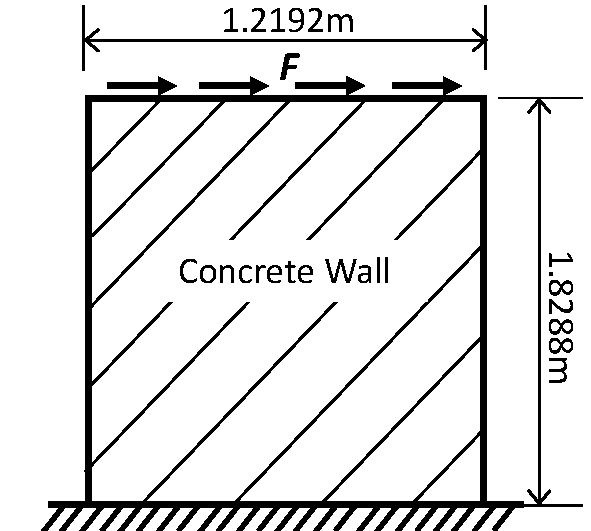
\includegraphics[width = 7cm]{./Figure-files/Day3/Wall_Pushover/overview.pdf}
  \caption{Illustrative Model of Wall Element Pushover Simulation }
  \label{fig_frame_pushover_wall}
\end{figure}


% ******************************************************************
% ******************************************************************
% ******************************************************************
\clearpage
\newpage
\section{ Viscous nonlinear behavior }
\label{Viscous_nonlinear_behavior}
% from small to very large

The Real-ESSI input files for this example are available 
\href{http://cml01.engr.ucdavis.edu/shortCourse/Day3/Viscous_nonlinear_behavior/Rayleigh}{HERE}. 
The compressed package of Real-ESSI input files for this example is available 
\href{http://cml01.engr.ucdavis.edu/shortCourse/Day3/Viscous_nonlinear_behavior/Rayleigh/Rayleigh.tgz}{HERE}. 


\begin{figure}[H]
  \centering
  \includegraphics[width = 0.5cm]{./Figure-files/Day3/Viscous_nonlinear_behavior/overview.png}
  \caption{Simulation Model}
  \label{fig_contact_examples1}
\end{figure}

The illustrative result is shown in Fig.~\ref{fig_day3_viscous_damping} and Fig.~\ref{fig_day3_viscous_damping_high}.

\begin{figure}[H]
  \centering
  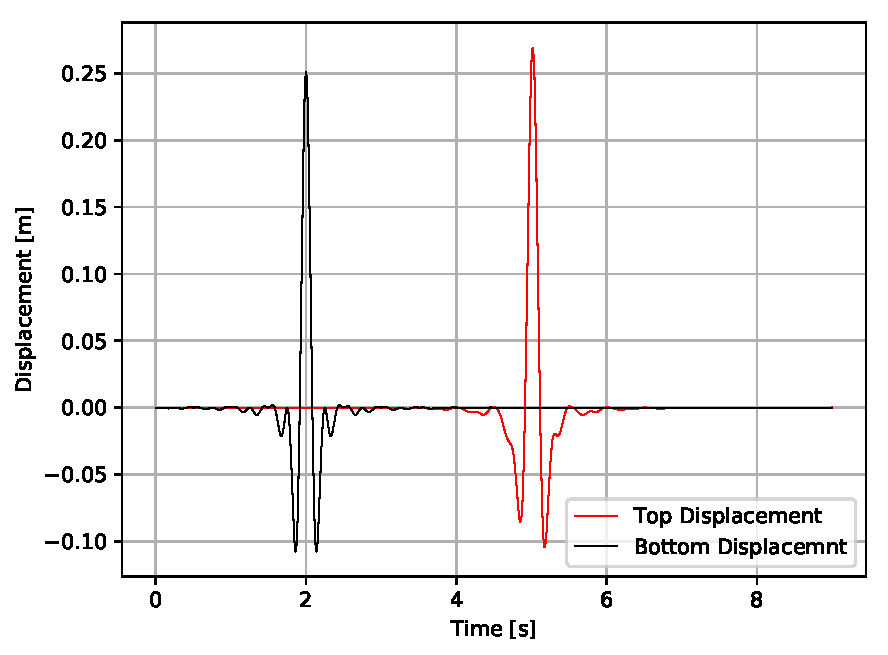
\includegraphics[width = 8cm]{./Figure-files/Day3/Viscous_nonlinear_behavior/Rayleigh001Displacement.pdf}
  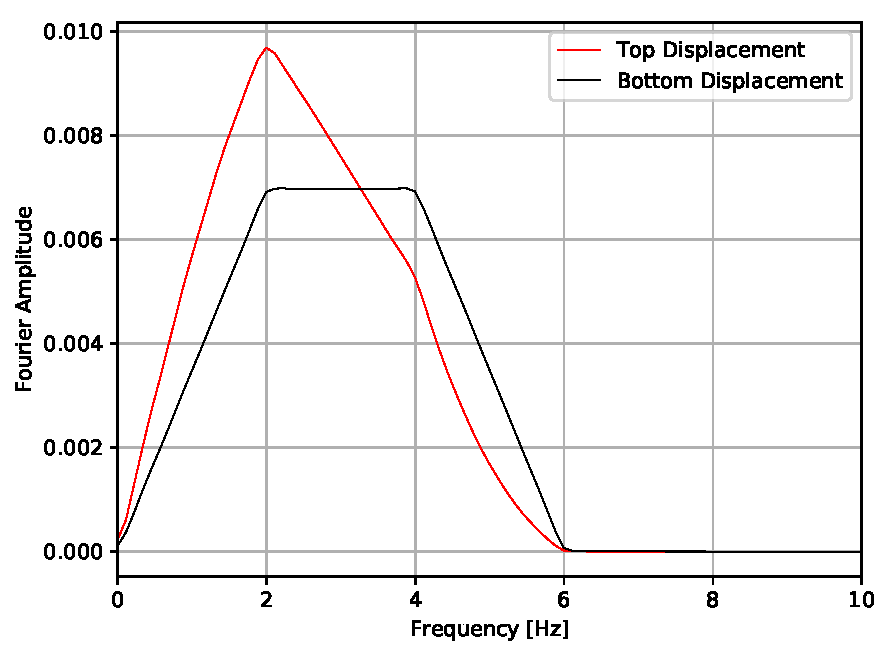
\includegraphics[width = 8cm]{./Figure-files/Day3/Viscous_nonlinear_behavior/Rayleigh001Displacement_Spectrum.pdf}
  \caption{Illustration results of Low Viscous Damping}
  \label{fig_day3_viscous_damping}
\end{figure}

\begin{figure}[H]
  \centering
  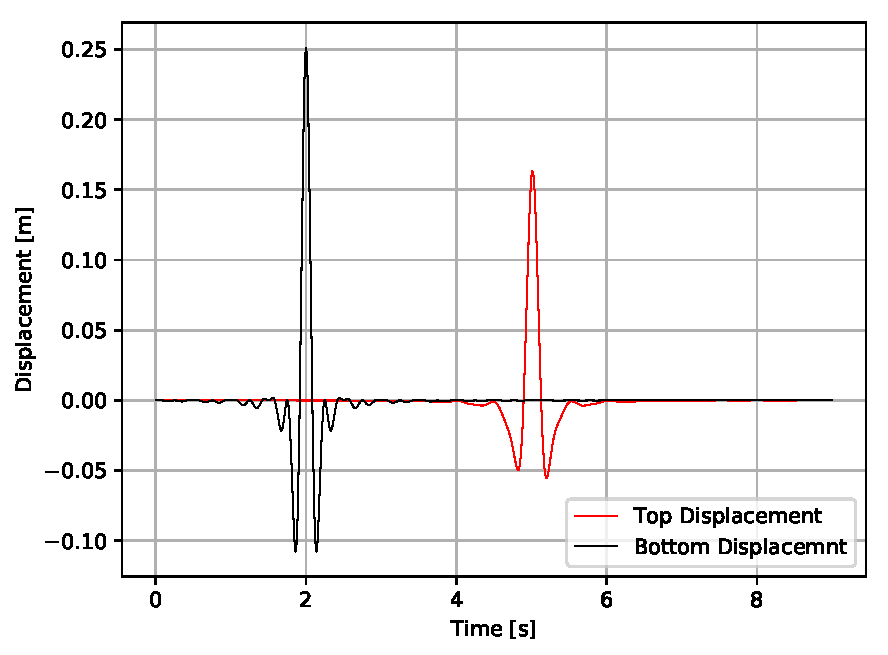
\includegraphics[width = 8cm]{./Figure-files/Day3/Viscous_nonlinear_behavior/Rayleigh002Displacement.pdf}
  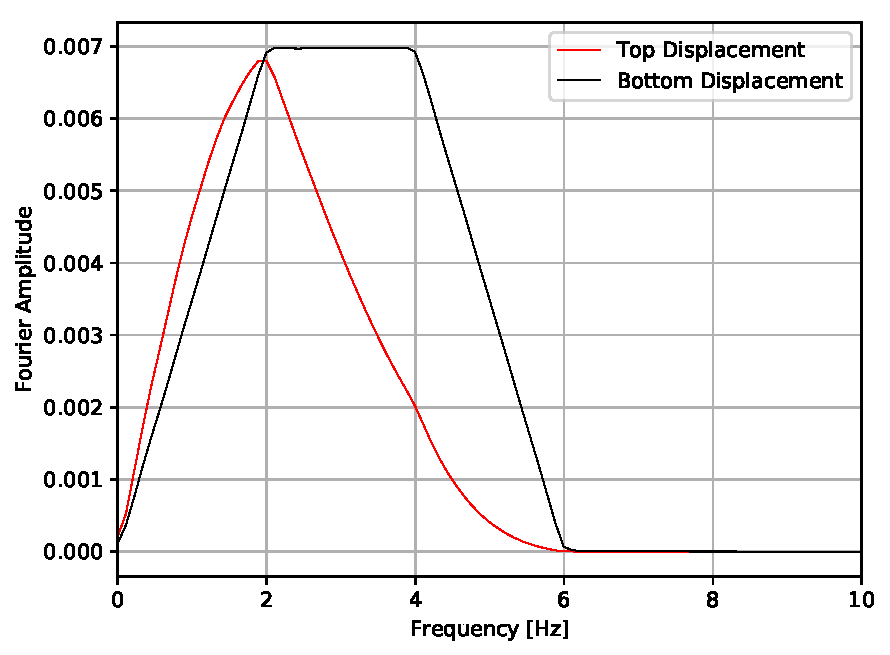
\includegraphics[width = 8cm]{./Figure-files/Day3/Viscous_nonlinear_behavior/Rayleigh002Displacement_Spectrum.pdf}
  \caption{Illustration results of High Viscous Damping}
  \label{fig_day3_viscous_damping_high}
\end{figure}




% ******************************************************************
% ******************************************************************
% ******************************************************************
\clearpage
\newpage
\section{ Numerical Damping Example }
\label{Numerical_Damping_Example}

The Real-ESSI input files for this example are available 
\href{http://cml01.engr.ucdavis.edu/shortCourse/Day3/Numerical_Damping_Example/newmark}{HERE}. 
The compressed package of Real-ESSI input files for this example is available 
\href{http://cml01.engr.ucdavis.edu/shortCourse/Day3/Numerical_Damping_Example/newmark/newmark.tgz}{HERE}. 


\begin{figure}[H]
  \centering
  \includegraphics[width = 0.5cm]{./Figure-files/Day3/Numerical_Damping_Example/overview.png}
  \caption{Simulation Model}
  \label{fig_contact_examples2}
\end{figure}


The illustrative result is shown in Fig.~\ref{fig_day3_viscous_damping} and Fig.~\ref{fig_day3_numerical_damping_high} .

\begin{figure}[H]
  \centering
  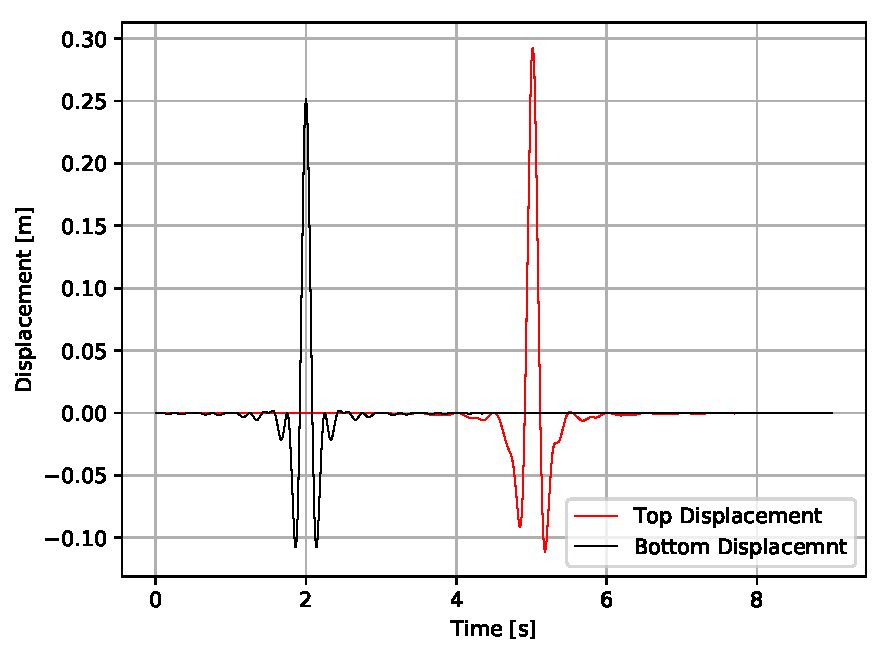
\includegraphics[width = 8cm]{./Figure-files/Day3/Numerical_Damping_Example/newmark06Displacement.pdf}
  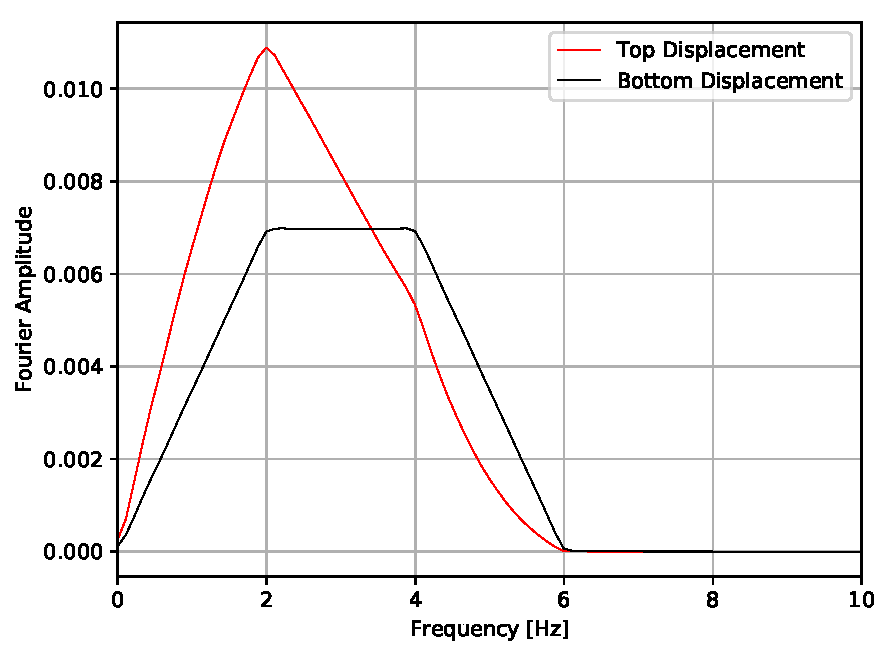
\includegraphics[width = 8cm]{./Figure-files/Day3/Numerical_Damping_Example/newmark06Displacement_Spectrum.pdf}
  \caption{Illustration results of Low numerical Damping}
  \label{fig_day3_numerical_damping}
\end{figure}

\begin{figure}[H]
  \centering
  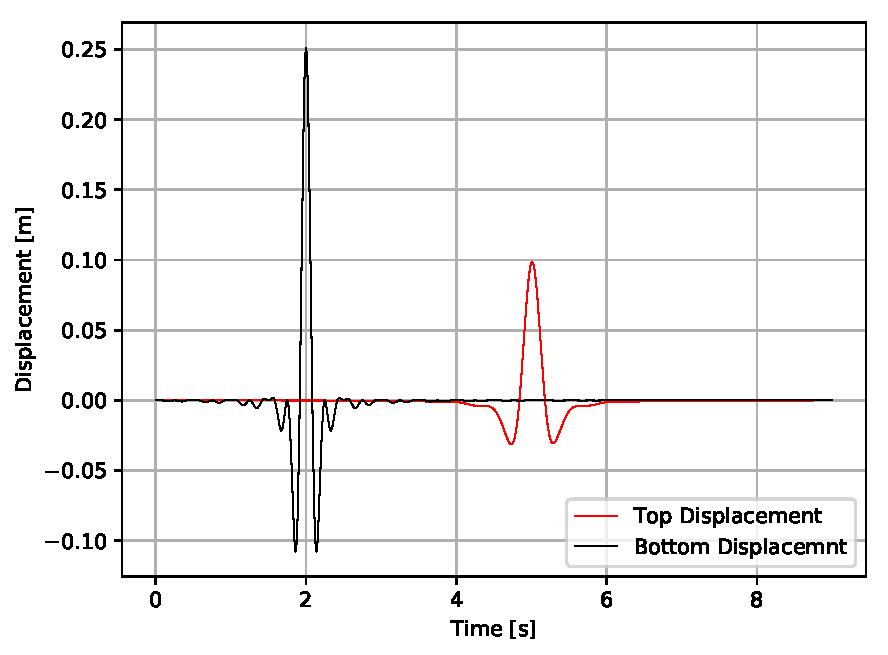
\includegraphics[width = 8cm]{./Figure-files/Day3/Numerical_Damping_Example/newmark10Displacement.pdf}
  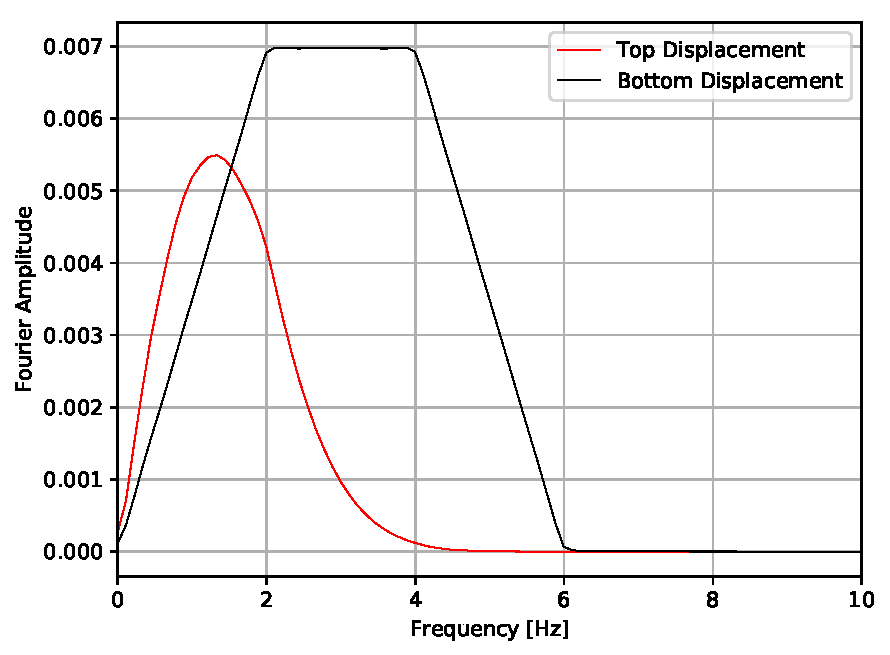
\includegraphics[width = 8cm]{./Figure-files/Day3/Numerical_Damping_Example/newmark10Displacement_Spectrum.pdf}
  \caption{Illustration results of High numerical Damping}
  \label{fig_day3_numerical_damping_high}
\end{figure}









% ******************************************************************
% ******************************************************************
% ******************************************************************
\clearpage
\newpage
\section{ Realistic Nuclear Power Plant Example with Nonlinearities}
\label{Realistic_Nuclear_Power_Plant_Example_with_Nonlinearities}


The Real-ESSI input files for this example are available 
\href{http://cml01.engr.ucdavis.edu/shortCourse/Day3/Realiastic_Nuclear_Power_Plant_Example_with_Nonlinearities}{HERE}. 
The compressed package of Real-ESSI input files for this example is available 
\href{http://cml01.engr.ucdavis.edu/shortCourse/Day3/Realiastic_Nuclear_Power_Plant_Example_with_Nonlinearities/Realiastic_Nuclear_Power_Plant_Example_with_Nonlinearities.tgz}{HERE}. 

The Modeling parameters are listed.
\begin{itemize}
  \item Soil 
  \begin{itemize}
    \item Unit weight, $\gamma$, \enspace \enspace 21.4 kPa
    \item Shear velocity, $Vs$, \enspace \enspace 500 m/s
    \item Young's modulus, $E$, \enspace \enspace 1.3 GPa
    \item Poisson's ratio, $\nu$, \enspace \enspace 0.25
    \item Shear strength, $S_u$, \enspace \enspace 650 kPa
    \item von Mises radius, $k$, \enspace \enspace 60 kPa
    \item kinematic hardening, $H_a$, \enspace \enspace 30 MPa
    \item kinematic hardening, $C_r$, \enspace \enspace 25
  \end{itemize}
  \item Structure
  \begin{itemize}
    \item Unit weight, $\gamma$, \enspace \enspace 24 kPa
    \item Young's modulus, $E$, \enspace \enspace 20 GPa
    \item Poisson's ratio, $\nu$, \enspace \enspace 0.21
  \end{itemize}
  \item Contact 
  \begin{itemize}
    \item Initial axial stiffness, $k_n^{init}$,  \enspace \enspace  1e9 N/m
    \item Stiffening rate, $S_r$,  \enspace \enspace  1000 /m 
    \item Maximum axial stiffness, $k_n^{max}$,  \enspace \enspace  1e12 N/m
    \item Shear stiffness, $k_t$,  \enspace \enspace  1e7 N/m
    \item Axial viscous damping, $C_n$,  \enspace \enspace  100 $N\cdot s /m$
    \item Shear viscous damping, $C_t$,  \enspace \enspace  100 $N\cdot s /m$
    \item Friction ratio, $\mu$,  \enspace \enspace  0.25
  \end{itemize}
\end{itemize}



\begin{figure}[H]
  \centering
  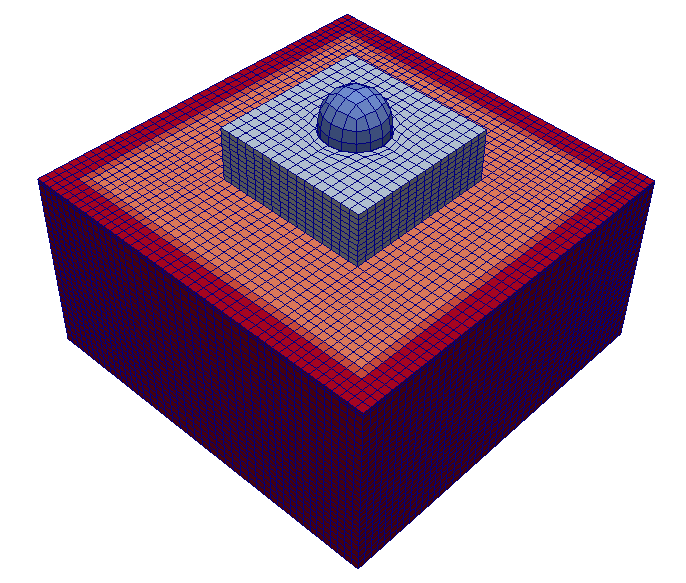
\includegraphics[width = 10cm]{./Figure-files/Day3/Realiastic_Nuclear_Power_Plant_Example_with_Nonlinearities/overview.png}
  \caption{Simulation Model}
  \label{fig_contact_examples3}
\end{figure}



SIMULATION TIME: With 32 cores on AWS EC2 c4.8xlarge instance, the running time for this example is 30 hours.